%definira klasu dokumenta 
\documentclass[12pt]{report} 

%prostor izmedu naredbi \documentclass i \begin{document} se zove uvod. U njemu se nalaze naredbe koje se odnose na cijeli dokument

%osnovni LaTex ne može riješiti sve probleme, pa se koriste različiti paketi koji olakšavaju izradu željenog dokumenta
\usepackage[croatian]{babel} 
\usepackage{amssymb}
\usepackage{amsmath}
\usepackage{txfonts}
\usepackage{mathdots}
\usepackage{titlesec}
\usepackage{array}
\usepackage{lastpage}
\usepackage{etoolbox}
\usepackage{tabularray}
\usepackage{color, colortbl}
\usepackage{adjustbox}
\usepackage{geometry}
\usepackage[classicReIm]{kpfonts}
\usepackage{hyperref}
\usepackage{fancyhdr}
\usepackage{ragged2e}
\usepackage{graphicx}
\usepackage{listings,lstautogobble}
\usepackage{xurl}
\graphicspath{ {./slike/} }

\usepackage{float}
\usepackage{setspace}
\restylefloat{table}

\patchcmd{\chapter}{\thispagestyle{plain}}{\thispagestyle{fancy}}{}{} %redefiniranje stila stranice u paketu fancyhdr

%oblik naslova poglavlja
\titleformat{\chapter}{\normalfont\huge\bfseries}{\thechapter.}{20pt}{\Huge}
\titlespacing{\chapter}{0pt}{0pt}{40pt}


\linespread{1.3} %razmak između redaka

\geometry{a4paper, left=1in, top=1in,}  %oblik stranice

\hypersetup{ colorlinks, citecolor=black, filecolor=black, linkcolor=black,	urlcolor=black }   %izgled poveznice


%prored smanjen između redaka u nabrajanjima i popisima
\newenvironment{packed_enum}{
	\begin{enumerate}
		\setlength{\itemsep}{0pt}
		\setlength{\parskip}{0pt}
		\setlength{\parsep}{0pt}
	}{\end{enumerate}}

\newenvironment{packed_item}{
	\begin{itemize}
		\setlength{\itemsep}{0pt}
		\setlength{\parskip}{0pt}
		\setlength{\parsep}{0pt}
	}{\end{itemize}}


%boja za privatni i udaljeni kljuc u tablicama
\definecolor{LightBlue}{rgb}{0.9,0.9,1}
\definecolor{LightGreen}{rgb}{0.9,1,0.9}

%Promjena teksta za dugačke tablice
\DefTblrTemplate{contfoot-text}{normal}{Nastavljeno na idućoj stranici}
\SetTblrTemplate{contfoot-text}{normal}
\DefTblrTemplate{conthead-text}{normal}{(Nastavljeno)}
\SetTblrTemplate{conthead-text}{normal}
\DefTblrTemplate{middlehead,lasthead}{normal}{Nastavljeno od prethodne stranice}
\SetTblrTemplate{middlehead,lasthead}{normal}

%podesavanje zaglavlja i podnožja

\pagestyle{fancy}
\lhead{Programsko inženjerstvo}
\rhead{Digitalizacija}
\lfoot{PiratesOfCode}
\cfoot{stranica \thepage/\pageref{LastPage}}
\rfoot{\today}
\renewcommand{\headrulewidth}{0.2pt}
\renewcommand{\footrulewidth}{0.2pt}


\begin{document} 
	
	
	
	\begin{titlepage}
		\begin{center}
			\vspace*{\stretch{1.0}} %u kombinaciji s ostalim \vspace naredbama definira razmak između redaka teksta
			\LARGE Programsko inženjerstvo\\
			\large Ak. god. 2021./2022.\\
			
			\vspace*{\stretch{3.0}}
			
			\huge Digitalizacija\\
			\Large Dokumentacija, Rev. \textit{2}\\
			
			\vspace*{\stretch{12.0}}
			\normalsize
			Grupa: \textit{PiratesOfCode}\\
			Voditelj: \textit{Ivan Futivić}\\
			
			
			\vspace*{\stretch{1.0}}
			Datum predaje: \textit{14. siječnja 2022.}\\
	
			\vspace*{\stretch{4.0}}
			
			Nastavnik: \textit{Igor Stančin}\\
		
		\end{center}

	
	\end{titlepage}

	
	\tableofcontents

	\chapter{Dnevnik promjena dokumentacije}
		
		\begin{longtblr}[
				label=none
			]{
				width = \textwidth, 
				colspec={|X[2]|X[13]|X[3]|X[3]|}, 
				rowhead = 1
			}
			\hline
			\textbf{Rev.}	& \textbf{Opis promjene/dodatka} & \textbf{Autori} & \textbf{Datum}\\[3pt] \hline
			0.1 & Dodani funkcionalni zahtjevi i obrasci uporabe& Blaž Solić & 22.10.2021. \\[3pt] \hline 
			0.1.1 & Dodani \textit{Use Case} dijagrami & Blaž Solić & 24.10.2021. \\[3pt] \hline 
			0.2 & Dodan opis projektnog zadatka & Luka Hanžek & 24.10.2021. \\[3pt] \hline 
			0.2.1 & Uređen i nadograđen opis projektnog zadatka& Luka Hanžek & 03.11.2021. \\[3pt] \hline
			0.3 & Dodani sekvencijalni dijagrami za registraciju i prijavu& Luka Hanžek & 03.11.2021. \\[3pt] \hline
			0.4 & Dodan opis i dijagram baze podataka& Blaž Solić& 10.11.2021. \\[3pt] \hline
			0.4.1 & Uređen dijagram baze podataka& Blaž Solić& 14.11.2021. \\[3pt] \hline
			0.5 & Dodan sekvencijalni dijagram za skeniranje & Luka Hanžek & 14.11.2021. \\[3pt] \hline
			0.6 & Dodan opis arhitekture& Blaž Solić& 17.11.2021. \\[3pt] \hline
			0.7 & Dodani dijagrami razreda& Karlo Marković& 17.11.2021. \\[3pt] \hline
			0.8 & Svi \textit{Use Case} dijagrami potpuno uređeni, preuređenje svih sekvencijalnih dijagram i dodavanje novih, dodani opisi sekvencijalnih dijagrama& Luka Hanžek& 18.11.2021. \\[3pt] \hline
			0.9 & Dodana nova klasa dijagramu razreda& Karlo Marković& 18.11.2021. \\[3pt] \hline
			0.9.1 & Dodani nefunkcionalni zahtjevi, opis projektnog zadatka potpuno uređen& Luka Hanžek& 19.11.2021. \\[3pt] \hline
			0.9.2 & Preuređeni dijagrami razreda& Karlo Marković& 19.11.2021. \\[3pt] \hline
			\textbf{1.0} & Verzija samo s bitnim dijelovima za 1. ciklus & Blaž Solić, Ivan Futivić, Luka Hanžek, Karlo Marković& 19.11.2021. \\[3pt] \hline 
			1.1 & Dodan dijagram stanja & Blaž Solić & 11.01.2022. \\[3pt] \hline
			1.2 & Izmijenjen dijagram baze & Blaž Solić & 11.01.2022. \\[3pt] \hline
			1.2.1 & Popravljen dijagram baze & Blaž Solić & 12.01.2022. \\[3pt] \hline
			1.3 & Dodane upute za puštanje u pogon & Ivan Futivić, Blaž Solić & 12.01.2022. \\[3pt] \hline
			1.4 & Izmijenjen dijagram stanja i dodana slika dijagrama baze & Blaž Solić & 12.01.2022. \\[3pt] \hline
			1.5 & Dodan dijagram razmještaja & Karlo Marković & 12.01.2022. \\[3pt] \hline
			1.6 & Popravljen dijagram razreda & Karlo Marković & 13.01.2022. \\[3pt] \hline
			1.6.1 & Dodane nove slike dijagrama razreda& Karlo Marković & 13.01.2022. \\[3pt] \hline
			1.7 & Dodan dijagram aktivnosti i slika & Karlo Kada & 14.01.2022. \\[3pt] \hline
			1.8 & Dodan dijagram komponenti & Luka Hanžek & 14.01.2022. \\[3pt] \hline
			1.9 & Opisano testiranje aplikacije & Nina Petrušić & 14.01.2022. \\[3pt] \hline
			1.10 & Opisane korištene tehnologije i alati & Ivan Futivić, Blaž Solić & 14.01.2022. \\[3pt] \hline
			1.11 & Dodana literatura & Luka Hanžek & 14.01.2022. \\[3pt] \hline 
			1.12 & Dodana zaključak i daljnji rad & Rafael Boban, Luka Hanžek & 14.01.2022. \\[3pt] \hline 
			2.0 & Konačna verzija dokumentacije & Ivan Futivić, Luka Hanžek, Karlo Marković, Nina Petrušić, Rafael Boban, Karlo Kada, Blaž Solić & 14.01.2022. \\[3pt] \hline

		\end{longtblr}
	
	\chapter{Opis projektnog zadatka}
		
		\section{Uvod}
		
		Rezultat ovog projektnog zadatka je mobilna aplikacija "SpyGlass"  i sustav namijenjen lakšoj internoj administraciji različitih tipova dokumenata unutar nekog poduzeća. Aplikacija će svim korisnicima unutar poslovnog subjekta pomoću ugrađene kamere na mobilnom uređaju omogućiti skeniranje dokumenata. Skenirani dokumenti će se pomoću optičkog prepoznavanje znakova pretvarati iz slikovnog formata u tekstualni format te će se u skladu s tipom dokumenta tekst na određeni način raščlaniti na dijelove. Dokumenti će se nakon skeniranja spremati u sustav i slati na daljnju obradu drugim korisnicima aplikacije zaduženim za određeni zadatak. Svaki korisnik će moći pristupiti svim već svojim skeniranim dokumentima, a ovisno o specijalizaciji korisnika aplikacija će korisniku nuditi i dodatne opcije. Korisnici aplikacije podijeljeni su u 4 kategorije koji tijekom rada sa sustavom međusobno razmjenjuju dokumente i tako administraciju dokumentima uvelike pojednostavljuju.
		
		\section{Korisnici aplikacije}
		Korisnici aplikacije svrstani su u četiri grupe od kojih svaka ima neke zajedničke i neke specifične mogućnosti. Korisnici aplikacije dijele se na sljedeće skupine: \underline{zaposlenik}, \underline{revizor}, \underline{računovođa} i \underline{direktor}. Korisnici se prije korištenja usluga moraju registrirati uz odabir određene specijalizacije. Prilikom registracije nužno je unijeti e-mail adresu, lozinku, specijalizaciju, ime i prezime. Ako korisnik odabire specijalizaciju računovođe, dodatno mora izabrati za koji tip dokumenta se opredjeljuje. Nakon uspješne registracije ili logiranja u sustav, korisnik ostaje zapamćen.

		\subsubsection{Zajedničke mogućnosti}
		Svi korisnici aplikacije imat će mogućnost skeniranja dokumenata pomoću ugrađene kamere na mobilnom uređaju te skenirani dokument potvrditi ili odbaciti, imati pristup svojim skeniranim dokumentima unutar same aplikacije i moći se registrirati ili prijaviti u aplikaciju ovisno o tome je li korisnik već registriran u sustavu ili nije.

		\subsubsection{Zaposlenik}
		Zadatak zaposlenika je skeniranje dokumenta te uz opciju skeniranja ima mogućnost preko gumba potvrditi ispravnost skeniranog dokumenta i tako poslati dokument na daljnju obradu revizoru ili ponovno skenirati isti dokument.

		\subsubsection{Revizor}
		Zadatak revizora je pregledavanje svih poslanih dokumenata od strane zaposlenika. Za svaki dobiveni dokument dužan je odrediti tip dokumenta i preusmjeriti ga računovođi koji je za taj tip dokumenta zadužen. Ako revizor skenira dokument, aplikacija automatski prepoznaje tip dokumenta.

		\subsubsection{Računovođa}
		Zadatak računovođe je arhiviranje dokumenata u bazu podataka. Dodatna opcija koju ima računovođa je slanje dokumenta na potpis direktoru prije arhiviranja. Nakon potpisa dokumenta računovođa dobiva obavijest da se dokument može arhivirati. Nakon otvaranja obavijesti, aplikacija automatski otvara dokument koji je potrebno potpisati i daje računovođi opciju za potpis.

		\subsubsection{Direktor}
		Zadatak direktora je potpisivanje dokumenata koje mu pošalje računovođa. Potpisivanje se može provesti preko obavijesti koju dobije kada računovođa pošalje dokument na potpisivanje ili preko odabira dokumenta iz liste koja prikazuje povijest skeniranih dokumenata spremnih za potpisivanje. Također ima mogućnost generirati i pregledavati statistike za sve zaposlenike i pregledavati povijest skeniranih dokumenata svih zaposlenika.
		
		\section{OCR skener}
		OCR (Optical Character Recognition) je glavna funkcionalnost aplikacije pomoću koje će se slike koje sadrže dokument skeniran pomoću kamere na mobilnom uređaju pretvarati iz slikovnog u tekstualni format. OCR skener dopušta skeniranje samo onda kada su ispunjena 2 uvjeta. Jedan od uvjeta je da je unutar vidnog polja prisutan dokument, a drugi da mobilni uređaj miruje minimalno 0.5 sekundi što se postiže praćenjem senzora mobilnog uređaja.
		\par
		Aplikacija pomoću OCR skenera uz samo skeniranje prepoznaje određeni tip dokumenta i na temelju izvornog teksta dokumenta izlučuje određeni sadržaj. Tipovi dokumenata koje OCR skener prepoznaje su: \underline{računi}, \underline{ponuda} i \underline{interni dokument}. Računi će u tekstu dokumenta imati oznaku koja se sastoji od velikog slova "R" te šest znamenaka, a sadržaj će se sastojati od imena klijenta, artikala s cijenama i ukupne cijene. Ponude će u tekstu dokumenta imati kao oznaku veliko slovo "P" i devet znamenaka, a sadržaj će se sastojati od artikala s cijenama i ukupne cijene. Interni dokument kao oznaku ima tri slova "INT" i četiri znamenke te nema određenu strukturu.
		
		\section{Ključni dijelovi sustava}
		Projekt će isporučiti javno dostupnu aplikaciju koja će se moći instalirati na većini suvremenih uređaja. Aplikacija zbog same prirode problematike koju rješava mora biti povezana na internet što uključuje bazu podataka koja mora podržavati veliki promet. Aplikacija zbog mogućnosti primanja obavijesti zahtjeva servis koji komunicira s bazom podataka u svrhu upravljanja obavijestima.
		

		\section{Slična rješenja}
		Sustav opisan ovdje trenutno na tržištu ne postoji, ali postoje brojne aplikacije koje imaju prevođenje slike dokumenata u tekstualni format i brojne druge usluge. Potražnja i vrijednost takvih aplikacija je velika i neupitna. Primjeri sličnih aplikacija dostupnih na tržištu su: CamScanner, OCR Text Scanner, Text Scanner i mnoge druge s preko 100 milijuna preuzimanja.
		%unos slike
		\begin{figure}[H]
			
\includegraphics[scale=0.7]{slike/CamScanner} %veličina slike u odnosu na originalnu datoteku i pozicija slike
			\centering
			\caption{ Primjer postojeće aplikacije}
			\label{fig:promjene}
		\end{figure}
		
	
	\chapter{Specifikacija programske potpore}
		
	\section{Funkcionalni zahtjevi}
			
			
			\noindent \textbf{Dionici:}
			
			\begin{packed_enum}
				
				\item Zaposlenik
				\item Revizor				
				\item Računovođa
				\item Direktor
				
			\end{packed_enum}
			
			\noindent \textbf{Aktori i njihovi funkcionalni zahtjevi:}
			
			
			\begin{packed_enum}
				\item  \underbar{Zaposlenik (inicijator) može:}
				
				\begin{packed_enum}
					
					\item skenirati dokument OCR-om
					\item vidjeti vlastitu povijest skeniranja
					\item poslati skenirani dokument revizoru ako je točno skeniran
					
				\end{packed_enum}
			
				\item  \underbar{Revizor (inicijator) može:}
				
				\begin{packed_enum}
					
					\item skenirati dokument OCR-om
					\item vidjeti vlastitu povijest skeniranja
					\item poslati skenirani dokument računovođama koji su za to namijenjeni
					
				\end{packed_enum}

                \item  \underbar{Računovođa (inicijator) može:}
				
				\begin{packed_enum}
					
					\item skenirati dokument OCR-om
					\item vidjeti vlastitu povijest skeniranja
					\item arhivirati dokumente ili ih poslati na potpisivanje direktoru
					\item primati direktorove obavijesti
					
				\end{packed_enum}

                \item  \underbar{Direktor (inicijator) može:}
				
				\begin{packed_enum}
					
					\item skenirati dokument OCR-om
					\item vidjeti vlastitu povijest skeniranja
					\item vidjeti povijest svih dokumenata svih korisnika
					\item vidjeti statistiku svih zaposlenika   
					\item primati računovođine obavijesti
					\item potpisivati dokumente
					
				\end{packed_enum}
			\end{packed_enum}
			
			\eject 
			
			
				
			\subsection{Obrasci uporabe}
				
				\subsubsection{Opis obrazaca uporabe}
					

					\noindent \underbar{\textbf{UC1 - Registracija}}
					\begin{packed_item}
	
						\item \textbf{Glavni sudionik:} Zaposlenik, revizor, računovođa, direktor
						\item  \textbf{Cilj:} Stvaranje stalnog računa te pristup onim funkcionalnostima aplikacije koje su korisniku potrebne
						\item  \textbf{Sudionici:} - Baza podataka
						\item  \textbf{Preduvjet:} - 
						\item  \textbf{Opis osnovnog tijeka:}
						
						\item[] \begin{packed_enum}
	
							\item Korisnik upisuje potrebne identifikacijske podatke
							\item Korisnik odabire specijalizaciju iz ponuđene liste dostupnih specijalizacija
							\item Korisnik biva obaviješten o registraciji
						\end{packed_enum}
						
						\item  \textbf{Opis mogućih odstupanja:}
						
						\item[] \begin{packed_item}
	
							\item[1.a]Korisnik upisuje podatke u neispravnom formatu 
							\item[] \begin{packed_enum}
								\item Sustav iznad krivo upisanog teksta navodi grešku
								\item Korisnik prepravlja unos prema uputama
							\end{packed_enum}
							\item[3.a]Korisnik je unio e-mail adresu koja već vezana za registriranog korisnika
							\item[] \begin{packed_enum}	
								\item Sustav obavještava korisnika o greški i vrača ga na ponovnu registraciju
								\item Korisnik unosi drugu e-mail adresu ili se prijavljuje sa zadnje unesenom
							\end{packed_enum}
						\end{packed_item}
					\end{packed_item}
					
					\noindent \underbar{\textbf{UC1.1: Odabir specijalizacije revizora}}
						\begin{packed_item}
		
							\item \textbf{Glavni sudionik:} Korisnik
							\item  \textbf{Cilj:} Odabir vrste dokumenta za kojeg će korisnik biti zadužen
							\item  \textbf{Sudionici:} - Baza podataka
							\item  \textbf{Preduvjet:} - Korisnik je na zaslonu registracije odabrao specijalizaciju računovođe
							\item  \textbf{Opis osnovnog tijeka:}
							
							\item[] \begin{packed_enum}
								\item Korisnik odabire za koji će tip dokumenta biti zadužen
							\end{packed_enum}
						\end{packed_item}

					\noindent \underbar{\textbf{UC2 - Prijava}}
						\begin{packed_item}
		
							\item \textbf{Glavni sudionik:} Zaposlenik, revizor, računovođa, direktor
							\item  \textbf{Cilj:} Prijava u sustav i početak korištenja usluga aplikacije
							\item  \textbf{Sudionici:} - Baza podataka
							\item  \textbf{Preduvjet:} - Korisnik je registriran
							\item  \textbf{Opis osnovnog tijeka:}
							
							\item[] \begin{packed_enum}
								\item Korisnik upisuje potrebne identifikacijske podatke
								\item Korisnik je preusmjeren na početni zaslon aplikacije
							\end{packed_enum}
							
							\item  \textbf{Opis mogućih odstupanja:}
							
							\item[] \begin{packed_item}
		
								\item[1.a]Korisnik upisuje neispravne podatke 
								\item[] \begin{packed_enum}
									\item Sustav u obliku pop-up teksta ispisuje poruku o neispravno unesenim podacima
									\item Korisnik prepravlja lozinku ili e-mail adresu
								\end{packed_enum}
							\end{packed_item}
						\end{packed_item}

					\noindent \underbar{\textbf{UC3 -  Odjava}}
						\begin{packed_item}
		
							\item \textbf{Glavni sudionik:} Zaposlenik, revizor, računovođa, direktor
							\item  \textbf{Cilj:} Odjava iz aplikacije u slučaju prijave drugog korisnika
							\item  \textbf{Sudionici:} - Baza podataka
							\item  \textbf{Preduvjet:} - Korisnik je prijavljen
							\item  \textbf{Opis osnovnog tijeka:}
							
							\item[] \begin{packed_enum}
								\item Korisnik odabire opciju "user info" na glavnom izborniku
								\item Korisnik se odjavljuje pritiskom na gumb za odjavu iz aplikacije
								\item Korisnik biva preusmjeren na zaslon aplikacije za prijavu
							\end{packed_enum}
						\end{packed_item}

					\noindent \underbar{\textbf{UC4 -  Skeniranje dokumenta}}
						\begin{packed_item}
		
							\item \textbf{Glavni sudionik:} Zaposlenik, revizor, računovođa, direktor
							\item  \textbf{Cilj:} Ispravno skenirati dokument te ga pohraniti u bazu podataka i u ovisnosti o specijalizaciji proslijediti ga drugom korisniku
							\item  \textbf{Sudionici:} - Baza podataka
							\item  \textbf{Preduvjet:} - Korisnik ima kameru na mobilnom uređaju
							\item  \textbf{Opis osnovnog tijeka:}
							
							\item[] \begin{packed_enum}
								\item Korisnik na glavnom izborniku odabire opciju "Scan"
								\item Korisnik uređaj pozicionira u skladu s dokumentom
								\item Korisnik čeka izvjesno vrijeme dok se uređaj ne stabilizira
								\item Korisnik pritiska gumb za okidanje slike
								\item Korisnik nakon provedenog OCR algoritma potvrđuje ispravnost skeniranja
								\item Korisnik o ovisnosti o specijalizaciji šalje dokument drugom korisniku ili ga arhivira
								\item Korisnik biva preusmjeren na zaslon spreman za ponovno skeniranje
							\end{packed_enum}
							
							\item  \textbf{Opis mogućih odstupanja:}
							
							\item[] \begin{packed_item}
		
								\item[1.a]Korisnik nema kameru na mobilnom uređaju 
								\item[] \begin{packed_enum}
									\item Na zaslonu se ispisuje poruka o nemogućnosti korištenja usluge skeniranja
								\end{packed_enum}
								\item[6.a]Korisnik nije zadovoljan skeniranim dokumentom
								\item[] \begin{packed_enum}
									\item Korisnik odabire opciju odbacivanja skeniranog dokumenta
									\item Korisnik ponovno skenira dokument
								\end{packed_enum}
							\end{packed_item}
						\end{packed_item}

					\noindent \underbar{\textbf{UC5 -  Pregled dokumenata}}
						\begin{packed_item}
		
							\item \textbf{Glavni sudionik:} Zaposlenik, revizor, računovođa, direktor
							\item  \textbf{Cilj:} Pregled onih dokumenata za koje je određeni korisnik odgovoran
							\item  \textbf{Sudionici:} - Baza podataka
							\item  \textbf{Preduvjet:} - Korisnik je prijavljen u sustav
							\item  \textbf{Opis osnovnog tijeka:}
							
							\item[] \begin{packed_enum}
								\item Korisnik na glavnom izborniku odabire opciju "History"
								\item Korisnik na temelju specijalizacije odabire opcije prikaza dokumenata
								\item Korisniku se prikazuju dokumenti
							\end{packed_enum}
							
							\item  \textbf{Opis mogućih odstupanja:}
							
							\item[] \begin{packed_item}
		
								\item[3.a]Korisnik za odabranu opciju nema dostupnih dokumenata
								\item[] \begin{packed_enum}
									\item Na zaslonu se umjesto popisa dokumenata ispsuje poruka
								\end{packed_enum}
							\end{packed_item}
						\end{packed_item}

					\noindent \underbar{\textbf{UC5.1 -  Pregled svih dokumenata}}
						\begin{packed_item}
		
							\item \textbf{Glavni sudionik:} Direktor
							\item  \textbf{Cilj:} Pregled svih skeniranih dokumenata svih korisnika
							\item  \textbf{Sudionici:} - Baza podataka
							\item  \textbf{Preduvjet:} - Korisnik je prijavljen u sustav i ima nivo autorizacije direktora
							\item  \textbf{Opis osnovnog tijeka:}
							
							\item[] \begin{packed_enum}
								\item Korisnik na glavnom izborniku odabire opciju "History"
								\item Korisnik iz izbornika filtera odabire opciju prikaza svih dokumenata
								\item Korisniku se prikazuju svi dokumenti svih korisnika
							\end{packed_enum}
							
							\item  \textbf{Opis mogućih odstupanja:}
							
							\item[] \begin{packed_item}
		
								\item[3.a]Korisnik za odabranu opciju nema dostupnih dokumenata
								\item[] \begin{packed_enum}
									\item Na zaslonu se umjesto popisa dokumenata ispsuje poruka
								\end{packed_enum}
							\end{packed_item}
						\end{packed_item}

					\noindent \underbar{\textbf{UC5.2 -  Pregled dokumenata za potpisivanje}}
						\begin{packed_item}
		
							\item \textbf{Glavni sudionik:} Direktor
							\item  \textbf{Cilj:} Pregled i potpisivanje dokumenata koje je prije arhiviranja potrebno potpisati
							\item  \textbf{Sudionici:} - Baza podataka
							\item  \textbf{Preduvjet:} - Korisnik je prijavljen u sustav i ima nivo autorizacije direktora
							\item  \textbf{Opis osnovnog tijeka:}
							
							\item[] \begin{packed_enum}
								\item Korisnik na glavnom izborniku odabire opciju "History"
								\item Korisnik iz izbornika filtera odabire opciju prikaza dokumenata za potpisivanje
								\item Korisniku se prikazuju svi dokumenti koji su spremni za potpisivanje
							\end{packed_enum}
							
							\item  \textbf{Opis mogućih odstupanja:}
							
							\item[] \begin{packed_item}
		
								\item[3.a]Korisnik za odabranu opciju nema dostupnih dokumenata
								\item[] \begin{packed_enum}
									\item Na zaslonu se umjesto popisa dokumenata ispsuje poruka
								\end{packed_enum}
							\end{packed_item}
						\end{packed_item}

					\noindent \underbar{\textbf{UC5.3 -  Pregled dokumenata za arhiviranje}}
						\begin{packed_item}
		
							\item \textbf{Glavni sudionik:} Računovođa
							\item  \textbf{Cilj:} Pregled svih dokumenata spremnih za arhiviranje
							\item  \textbf{Sudionici:} - Baza podataka
							\item  \textbf{Preduvjet:} - Korisnik je prijavljen u sustav i ima nivo autorizacije računovođe
							\item  \textbf{Opis osnovnog tijeka:}
							
							\item[] \begin{packed_enum}
								\item Korisnik na glavnom izborniku odabire opciju "History"
								\item Korisnik iz izbornika filtera odabire opciju prikaza dokumenata spremnih za arhiviranje
								\item Korisniku se prikazuju svi dokumenti spremni za arhiviranje
							\end{packed_enum}
							
							\item  \textbf{Opis mogućih odstupanja:}
							
							\item[] \begin{packed_item}
		
								\item[3.a]Korisnik za odabranu opciju nema dostupnih dokumenata
								\item[] \begin{packed_enum}
									\item Na zaslonu se umjesto popisa dokumenata ispsuje poruka
								\end{packed_enum}
							\end{packed_item}
						\end{packed_item}

					\noindent \underbar{\textbf{UC5.4 -  Pregled dokumenata za reviziju}}
						\begin{packed_item}
		
							\item \textbf{Glavni sudionik:} Revizor
							\item  \textbf{Cilj:} Pregled dokumenata spremnih za reviziju
							\item  \textbf{Sudionici:} - Baza podataka
							\item  \textbf{Preduvjet:} - Korisnik je prijavljen u sustav i ima nivo autorizacije revizora
							\item  \textbf{Opis osnovnog tijeka:}
							
							\item[] \begin{packed_enum}
								\item Korisnik na glavnom izborniku odabire opciju "History"
								\item Korisnik iz izbornika filtera odabire opciju prikaza dokumenata spremnih za reviziju
								\item Korisniku se prikazuju svi dokumenti svih korisnika
							\end{packed_enum}
							
							\item  \textbf{Opis mogućih odstupanja:}
							
							\item[] \begin{packed_item}
		
								\item[3.a]Korisnik za odabranu opciju nema dostupnih dokumenata
								\item[] \begin{packed_enum}
									\item Na zaslonu se umjesto popisa dokumenata ispsuje poruka
								\end{packed_enum}
							\end{packed_item}
						\end{packed_item}

					\noindent \underbar{\textbf{UC5.5 -  Pregled vlastito skeniranih dokumenata}}
						\begin{packed_item}
		
							\item \textbf{Glavni sudionik:} Zaposlenik, revizor, računovođa, direktor
							\item  \textbf{Cilj:} Pregled svih dokumenata koje je skenirao trenutno prijavljeni korisnik
							\item  \textbf{Sudionici:} - Baza podataka
							\item  \textbf{Preduvjet:} - Korisnik je prijavljen u sustav
							\item  \textbf{Opis osnovnog tijeka:}
							
							\item[] \begin{packed_enum}
								\item Korisnik na glavnom izborniku odabire opciju "History"
								\item Korisnik iz izbornika filtera odabire opciju prikaza svih vlastito skeniranih
								\item Korisniku se prikazuju svi dokumenti svih korisnika
							\end{packed_enum}
							
							\item  \textbf{Opis mogućih odstupanja:}
							
							\item[] \begin{packed_item}
		
								\item[3.a]Korisnik za odabranu opciju nema dostupnih dokumenata
								\item[] \begin{packed_enum}
									\item Na zaslonu se umjesto popisa dokumenata ispsuje poruka
								\end{packed_enum}
							\end{packed_item}
						\end{packed_item}

					\noindent \underbar{\textbf{UC6 - Pregled korisničkih podataka}}
						\begin{packed_item}
		
							\item \textbf{Glavni sudionik:} Zaposlenik, revizor, računovođa, direktor
							\item  \textbf{Cilj:} Pregled korisničkih podataka vezanih za trenutno prijavljenog korisnika
							\item  \textbf{Sudionici:} - Baza podataka
							\item  \textbf{Preduvjet:} - Korisnik je prijavljen u sustav
							\item  \textbf{Opis osnovnog tijeka:}
							
							\item[] \begin{packed_enum}
								\item Korisnik na glavnom izborniku odabire opciju "Info"
								\item Korisniku se prikazuju korisnički podaci
							\end{packed_enum}
						\end{packed_item}

					\noindent \underbar{\textbf{UC7 - Slanje dokumenta revizoru}}
						\begin{packed_item}
		
							\item \textbf{Glavni sudionik:} Zaposlenik
							\item  \textbf{Cilj:} Slanje skeniranog dokumenta odgovarajućem korisniku u svrhu daljnje obrade
							\item  \textbf{Sudionici:} - Baza podataka
							\item  \textbf{Preduvjet:} - Korisnik je prijavljen u sustav i ima nivo autorizacije zaposlenika
							\item  \textbf{Opis osnovnog tijeka:}
							
							\item[] \begin{packed_enum}
								\item Korisnik na glavnom izborniku odabire opciju "scan"
								\item Korisnik skenira dokument
								\item Korisniku potvrđuje kvalitetu skeniranog dokumenta
								\item Korisnik šalje dokument revizoru
							\end{packed_enum}
						\end{packed_item}

					\noindent \underbar{\textbf{UC8 - Slanje dokumenta računovođi}}
						\begin{packed_item}
		
							\item \textbf{Glavni sudionik:} Revizor
							\item  \textbf{Cilj:} Slanje dokumenta računovođama koji su zaduženi za određeni tip skeniranog dokumenta
							\item  \textbf{Sudionici:} - Baza podataka
							\item  \textbf{Preduvjet:} - Korisnik je prijavljen i ima nivo autorizacije revizora
							\item  \textbf{Opis osnovnog tijeka:}
							
							\item[] \begin{packed_enum}
								\item Korisnik prilikom pregleda dokumenata odabire dokument spreman za reviziju
								\item Korisnik odabire tip dokumenta kako bi dokument bio proslijeđen ispravnim računovođama
							\end{packed_enum}
							
							\item  \textbf{Opis mogućih odstupanja:}
							
							\item[] \begin{packed_item}
		
								\item[1.a]Korisnik kod pregleda dokumenata za odabranu opciju nema dostupnih dokumenata
								\item[] \begin{packed_enum}
									\item Na zaslonu se umjesto popisa dokumenata ispsuje poruka
								\end{packed_enum}
							\end{packed_item}

							\item  \textbf{Alternativni tijek:}

							\item[] \begin{packed_item}
		
								\item[1.a]Korisnik skenira dokument
								\item[2.a]Ako je korisnik skenirao dokument, aplikacija sama prepoznaje tip dokumenta
							\end{packed_item}
						\end{packed_item}
					\noindent \underbar{\textbf{UC9 - Arhiviranje dokumenata}}
						\begin{packed_item}
		
							\item \textbf{Glavni sudionik:} Računovođa
							\item  \textbf{Cilj:} Spremanje potpuno obrađenih dokumenata u bazu podataka
							\item  \textbf{Sudionici:} - Baza podataka
							\item  \textbf{Preduvjet:} - Korisnik je prijavljen u sustav i ima nivo autorizacije računovođe
							\item  \textbf{Opis osnovnog tijeka:}
							
							\item[] \begin{packed_enum}
								\item Korisnik odabire pregled dokumenata
								\item Korisnik odabire opciju prikaza dokumenata dostupnih za arhiviranje
								\item Korisnik odabire dokument koji želi arhivirati
								\item Korisnik arhivira zadani dokument
							\end{packed_enum}
							
							\item  \textbf{Alternativni tijek:}

							\item[] \begin{packed_item}
		
								\item[1-3.a]Korisnik dobiva obavijest
								\item[] \begin{packed_enum}
									\item Korisnik pritiskom na obavijest dolazi do zaslona na kojem se prikazuje dokument
								\end{packed_enum}
							\end{packed_item}
						\end{packed_item}

					\noindent \underbar{\textbf{UC10 - Slanje dokumenta na potpis}}
						\begin{packed_item}
		
							\item \textbf{Glavni sudionik:} Računovođa
							\item  \textbf{Cilj:} Pregled svih skeniranih dokumenata svih korisnika
							\item  \textbf{Sudionici:} - Baza podataka
							\item  \textbf{Preduvjet:} - Korisnik je prijavljen u sustav i ima nivo autorizacije računovođe
							\item  \textbf{Opis osnovnog tijeka:}
							
							\item[] \begin{packed_enum}
								\item Korisnik odabire opciju "History"
								\item Korisnik iz izbornika filtera odabire opciju prikaza dokumenata za potpis
								\item Korisnik odabire dokument koji želi poslati na potpis
								\item korisnik šalje dokument na potpis
							\end{packed_enum}

							\item  \textbf{Alternativni tijek:}

							\item[] \begin{packed_item}
		
								\item[1-3.a]Korisnik skenira dokument
								\item[] \begin{packed_enum}
									\item Korisnik odabire opciju "Scan"
									\item Korisnik skenira dokument
									\item Korisnik potvrđuje kvalitetu skeniranog dokumenta
									\item Korisnik odabire opciju slanja dokumenta na potpis
								\end{packed_enum}
								\item  \textbf{Opis mogućih odstupanja:}
							
								\item[] \begin{packed_item}
			
									\item[4.]Korisnik odabire opciju arhiviranja dokumenta
									\item[] \begin{packed_enum}
										\item Korisnik biva prebačen na zaslon skeniranja
									\end{packed_enum}
								\end{packed_item}
							\end{packed_item}
						\end{packed_item}

					\noindent \underbar{\textbf{UC11 - Primanje obavijesti}}
						\begin{packed_item}
		
							\item \textbf{Glavni sudionik:} Direktor, računovođa
							\item  \textbf{Cilj:} Brzi pristup dokumentu kojega je potrebno obraditi
							\item  \textbf{Sudionici:} - Baza podataka
							\item  \textbf{Preduvjet:} - Korisniku je poslan dokument od strane drugog korisnika
							\item  \textbf{Opis osnovnog tijeka:}
							
							\item[] \begin{packed_enum}
								\item Korisnik otvara obavijest
								\item Korisnik biva preusmjeren na zaslon koji sadrži podatke o dokumentu
								\item Korisnik obrađuje dokument na način na koji je za to zadužen
							\end{packed_enum}
							
							\item  \textbf{Opis mogućih odstupanja:}
							
							\item[] \begin{packed_item}
		
								\item[1.a]Korisnik briše obavijest
								\item[] \begin{packed_enum}
									\item Korisnik nastavlja rad, a dokument se obrađuje klikom na određeni dokument na zaslonu pregleda dokumenata
								\end{packed_enum}
							\end{packed_item}
						\end{packed_item}

					\noindent \underbar{\textbf{UC12 - Potpisivanje dokumenta}}
						\begin{packed_item}
		
							\item \textbf{Glavni sudionik:} Direktor
							\item  \textbf{Cilj:} Označavanje dokumenta potpisanim
							\item  \textbf{Sudionici:} - Baza podataka
							\item  \textbf{Preduvjet:} - Korisnik je prijavljen u sustav i ima nivo autorizacije direktora
							\item  \textbf{Opis osnovnog tijeka:}
							
							\item[] \begin{packed_enum}
								\item Korisnik na glavnom izborniku odabire opciju "History"
								\item Korisnik iz izbornika filtera odabire opciju prikaza dokumenata za potpisivanje
								\item Korisniku se prikazuju svi dokumenti za potpisivanje
								\item Korisnik odabire dokument koji želi potpisati
								\item Korisniku se prikazuju podaci odabranog dokumenta
								\item Korisnik potpisuje dokument
							\end{packed_enum}
							
							\item  \textbf{Opis mogućih odstupanja:}
							
							\item[] \begin{packed_item}
		
								\item[4.a]Dokument je već potpisan od strane drugog računovođe
								\item[] \begin{packed_enum}
									\item Korisnik nastavlja rad
								\end{packed_enum}
							\end{packed_item}

							\item  \textbf{Alternativni koraci:}

							\item[] \begin{packed_item}
		
								\item[1-4.a]Korisnik je dobio obavijest
								\item[] \begin{packed_enum}
									\item Korisnik pritišće na obavijest
									\item Korisniku se prikazuju podaci dokumenta referenciranog u obavijesti
								\end{packed_enum}
							\end{packed_item}
						\end{packed_item}

					\noindent \underbar{\textbf{UC13 - Pregled statistike}}
						\begin{packed_item}
		
							\item \textbf{Glavni sudionik:} Direktor
							\item  \textbf{Cilj:} Uvid u statistiku zaposlenika
							\item  \textbf{Sudionici:} - Baza podataka
							\item  \textbf{Preduvjet:} - Korisnik je prijavljen u sustav i ima nivo autorizacije direktora
							\item  \textbf{Opis osnovnog tijeka:}
							
							\item[] \begin{packed_enum}
								\item Korisnik na glavnom izborniku odabire opciju "Info"
								\item Korisnik odabire opciju "Statistics"
								\item Korisniku se prikazuje lista svih zaposlenika
								\item Korisnik odabire zaposlenika za kojega želi prikazati statistiku
								\item Korisniku se prikazuje zaslon s odgovarajućom statistikom
							\end{packed_enum}
						\end{packed_item}
				\subsubsection{Dijagrami obrazaca uporabe}
				
				
				%unos slike
				\begin{figure}[H]
					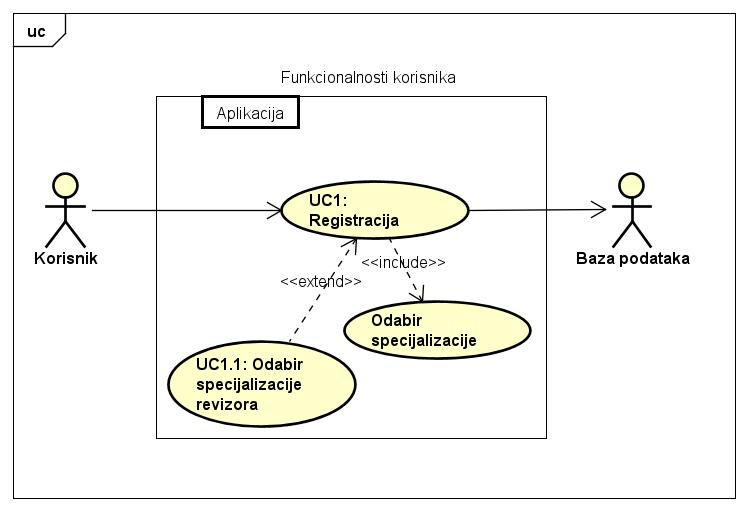
\includegraphics[scale=0.5]{slike/Funkcionalnosti korisnika} %veličina slike u odnosu na originalnu datoteku i pozicija slike
					\centering
					\caption{ Dijagram obrasca uporabe, funkcionalnosti korisnika}
					\label{fig:promjene}
				\end{figure}

				%unos slike
				\begin{figure}[H]
					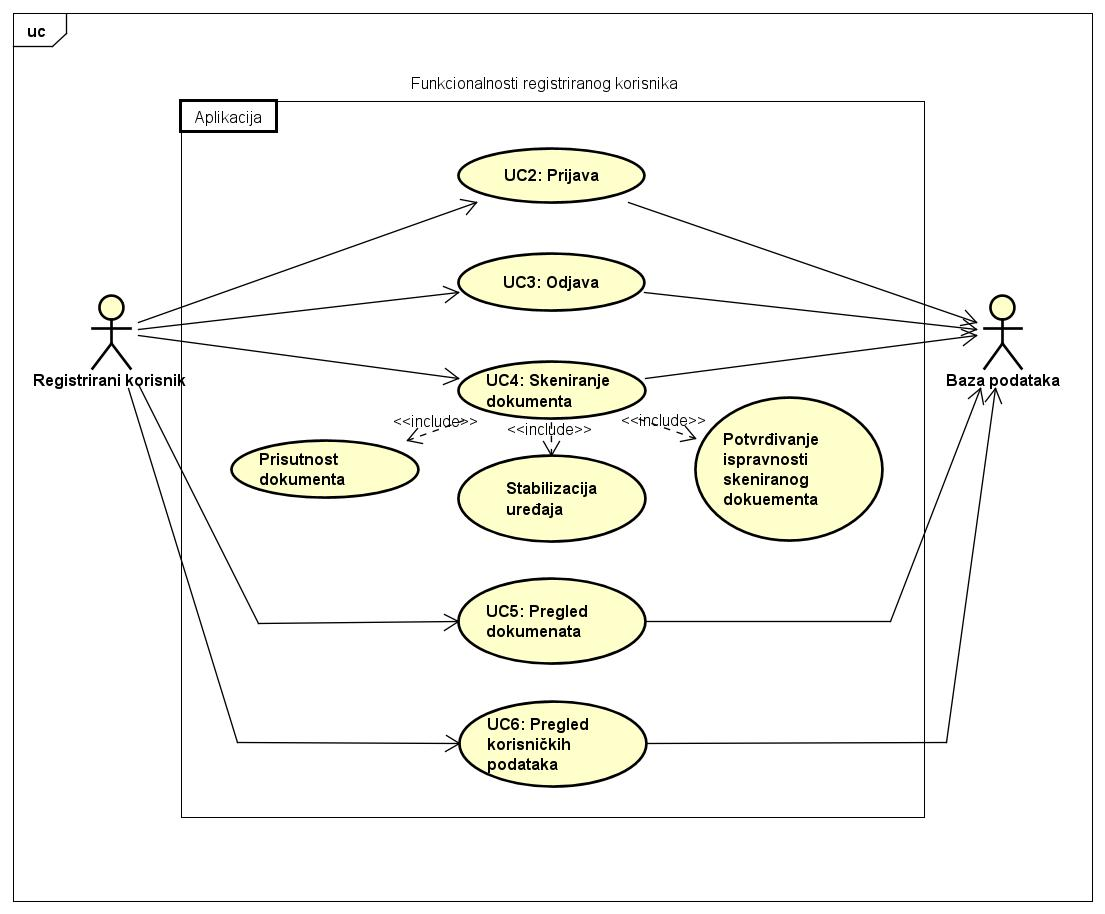
\includegraphics[scale=0.4]{slike/Funkcionalnosti registriranog korisnika} %veličina slike u odnosu na originalnu datoteku i pozicija slike
					\centering
					\caption{ Dijagram obrasca uporabe, funkcionalnosti registriranog korisnika}
					\label{fig:promjene}
				\end{figure}

				%unos slike
				\begin{figure}[H]
					\includegraphics[scale=0.4]{slike/funkcionalnosti specijalizacija} %veličina slike u odnosu na originalnu datoteku i pozicija slike
					\centering
					\caption{ Dijagram obrasca uporabe, funkcionalnosti specijalizacija}
					\label{fig:promjene}
				\end{figure}

				%unos slike
				\begin{figure}[H]
					\includegraphics[scale=0.3]{slike/pregled dokumenata} %veličina slike u odnosu na originalnu datoteku i pozicija slike
					\centering
					\caption{ Dijagram obrasca uporabe, pregled dokumenata}
					\label{fig:promjene}
				\end{figure}
				\eject		
				
			\subsection{Sekvencijski dijagrami}


				\subsubsection{Obrazac uporabe UC1 - Registracija}
				Korisnik otvara aplikaciju te mu aplikacija u slučaju da nitko na uređaju nije prijavljen u sustav prikazuje zaslon za registraciju novog korisnika. Dok korisnik unosi identifikacijske podatke aplikacija konstantno provjerava ispravnost formata unesenih podataka kao što je dovoljno jaka lozinka ili ispravan format e-mail adrese te u slučaju detektiranja greške ispisuje odgovarajuću poruku iznad polja u kojem je greška. Nakon što korisnik unese podatke ispravnog formata, pritišće gumb za registraciju. Ako se je korisnik specijalizirao kao računovođa, aplikacija mu ispisuje izbornik sa svim tipovima dokumenata koji su dostupni. Korisnik odabire dokument za koji će biti zadužen te potvrđuje odabir. Aplikacija unesene podatke šalje u bazu podataka gdje se podaci provjeravaju. Ako baza podataka ustanovi da korisnik s istom e-mail adresom već postoji, registracija se odbacuje i korisniku se ispisuje odgovarajuća poruka. Ako je registracija uspjela, korisnik biva preusmjeren na početni zaslon aplikacije.
				%unos slike
				\begin{figure}[H]
					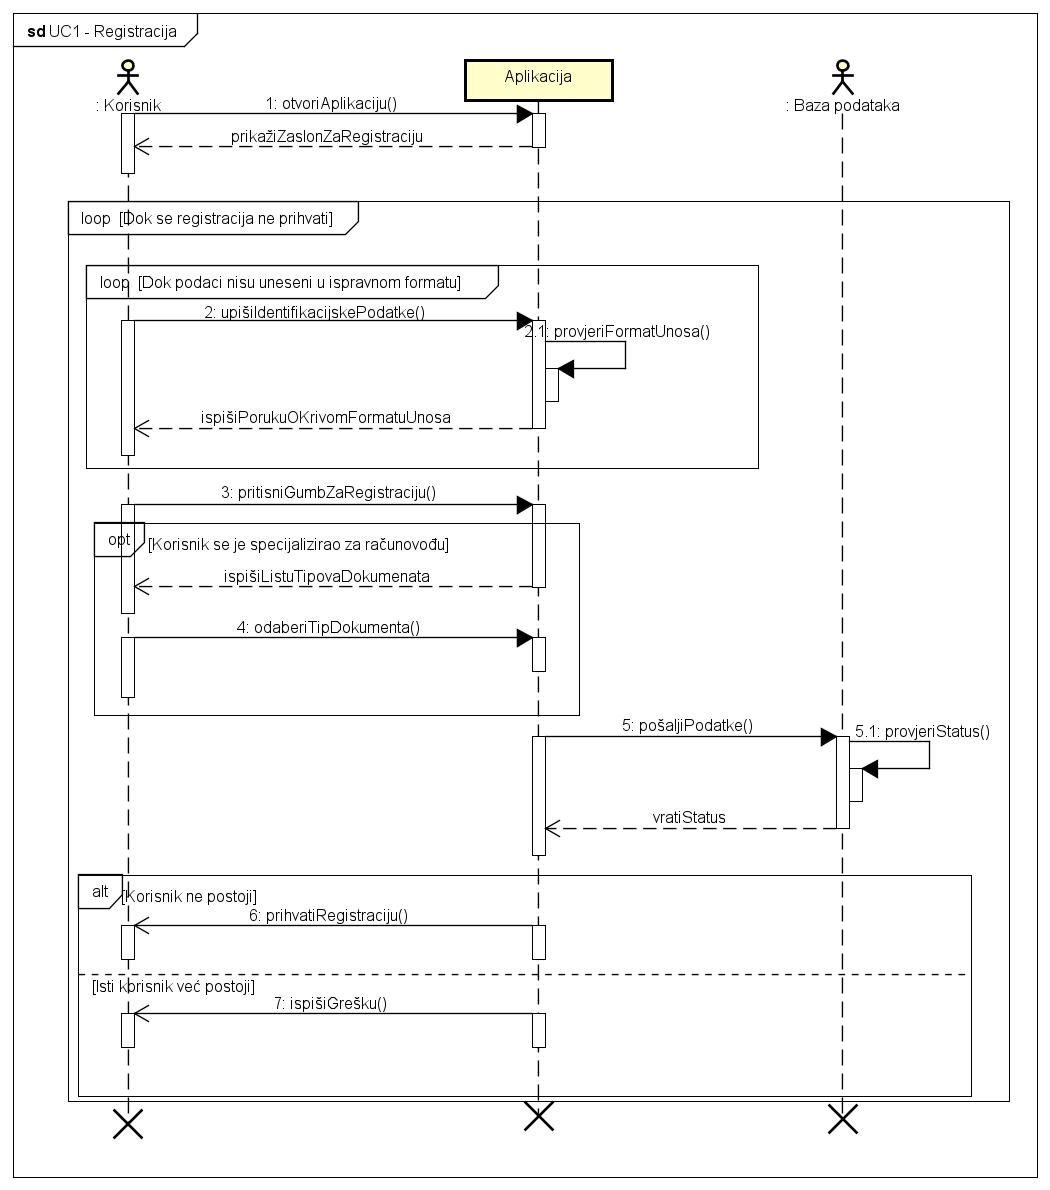
\includegraphics[scale=0.35]{slike/UC1 - Registracija} %veličina slike u odnosu na originalnu datoteku i pozicija slike
					\centering
					\caption{ Sekvencijalni dijagram, UC1}
					\label{fig:promjene}
				\end{figure}

				\subsubsection{Obrazac uporabe UC4 - Skeniranje}
				Korisnik na glavnom izborniku odabire opciju skeniranja te mu aplikacija na zaslonu prikazuje pogled kamere. Aplikacija korisniku ne dozvoljava skeniranje prije nego što su zadovoljena dva uvjeta. Prvi uvjet je da se u pogledu kamere nalazi dokument. Drugi uvjet je ispunjen kada aplikacija u određenom periodu vremena ne izmjeri vibracije sa senzora na mobilnom uređaju. Kada je dokument prisutan i uređaj je stabilan, aplikacija korisniku omogućuje okidanje fotografije. Aplikacija nakon okidanja fotografije izvodi OCR algoritam. Nakon izvedenog algoritma aplikacija korisniku daje opciju prihvaćanja ili odbacivanja skeniranog dokumenta na temelju kvalitete skeniranja. Ako korisnik odbaci skenirani dokument, aplikacija dokument pohranjuje u bazu podataka s oznakom da je neispravno skeniran. Ako korisnik prihvati skenirani dokument, aplikacija u bazu podataka pohranjuje dokument s oznakom da je ispravno skeniran.
				%unos slike
				\begin{figure}[H]
					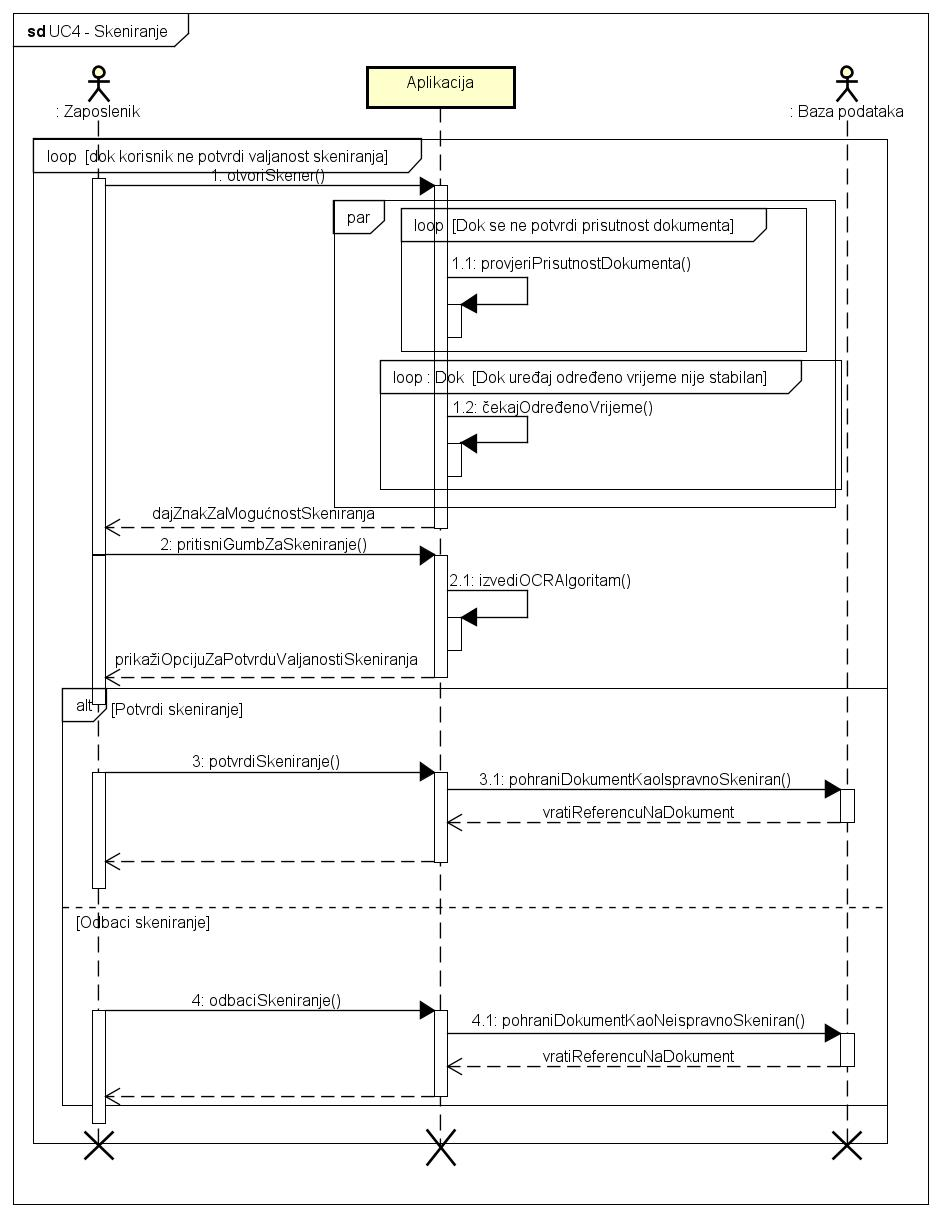
\includegraphics[scale=0.35]{slike/UC4 - Skeniranje} %veličina slike u odnosu na originalnu datoteku i pozicija slike
					\centering
					\caption{ Sekvencijalni dijagram, UC4}
					\label{fig:promjene}
				\end{figure}


				\subsubsection{Obrazac uporabe UC8 - Slanje dokumenta računovođi}
				Revizor dokument računovođi na arhiviranje može poslati na dva načina. U slučaju da računovođi treba poslati dokument koji je već skeniran od strane zaposlenika, revizor u pregledu dokumenata odabire filtar za prikaz dokumenata spremnih za slanje računovođi. Aplikacija iz baze podataka dohvaća tražene dokumente i prikazuje ih revizoru. Revizor na izborniku odabire željeni dokument. Aplikacija otvara izabrani dokument i prikazuje ga revizoru. Revizor odabire opciju slanja dokumenta računovođi. Budući da je svaki računovođa zadužen za određeni tip dokumenta, aplikacija revizoru prikazuje izbornik koji sadrži popis svih tipova dokumenta. Revizor izabire onaj tip dokumenta koji odgovara skeniranom dokumentu. Aplikacija u bazi podataka mijenja status dokumenta što dokument čini vidljivim računovođi. Revizor ponavlja radnju sve dok ne pošalje sve željene dokumente. \par U slučaju da revizor treba poslati dokument kojeg još nije skenirao zaposlenik, revizor treba skenirati dokument sam. Nakon skeniranja aplikacija dokumentu automatski odredi tip i pohrani ga u bazu podataka.
				%unos slike
				\begin{figure}[H]		
					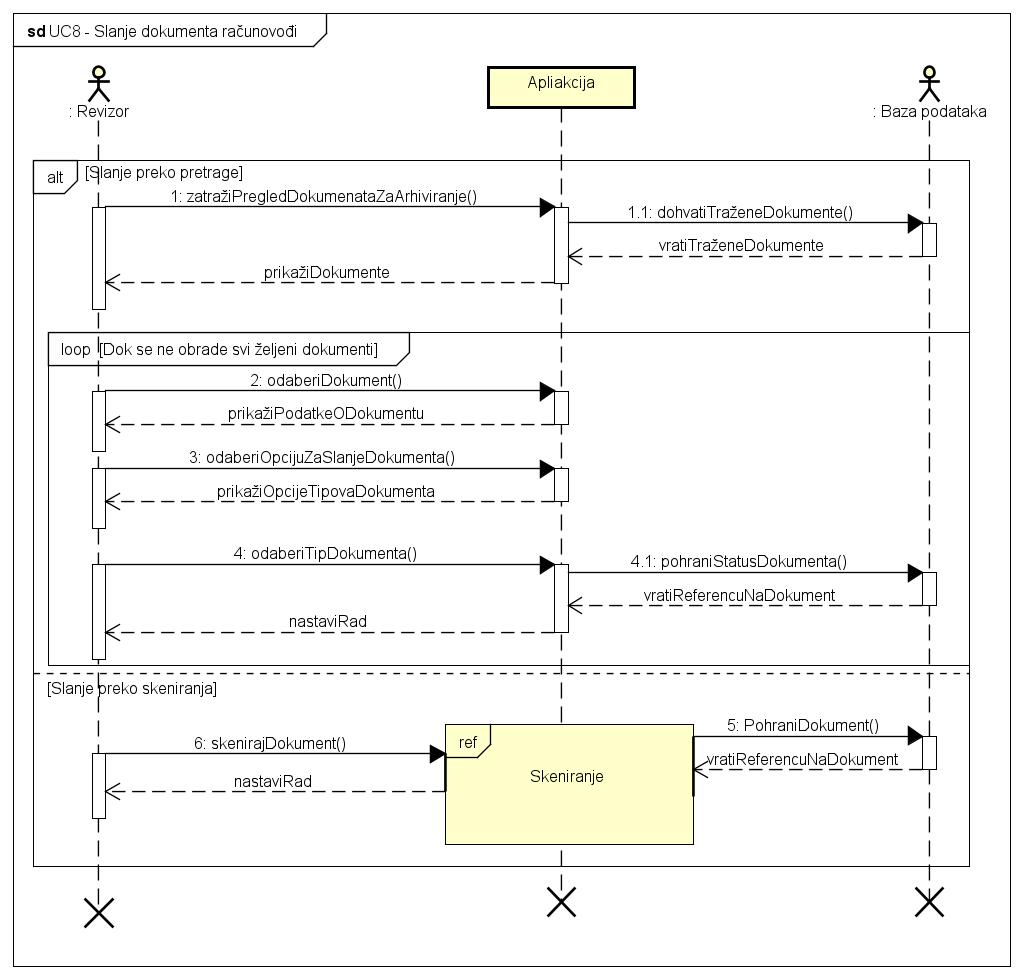
\includegraphics[scale=0.35]{slike/UC8 - Slanje dokumenta računovođi} %veličina slike u odnosu na originalnu datoteku i pozicija slike
					\centering
					\caption{ Sekvencijalni dijagram, UC8}
					\label{fig:promjene}
				\end{figure}

				\subsubsection{Obrazac uporabe UC12 - Potpisivanje dokumenata}
				Računovođa dokument može potpisati na dva načina. Jedan način je da direktor nakon što računovođa pošalje dokument na potpisivanje dobije obavijest. Aplikacija direktoru prikazuje obavijest na alatnoj traci mobilnog uređaja. Nakon što direktor otvara obavijest, aplikacija dohvaća dokument referenciran u obavijesti iz baze podataka i prikazuje ga na zaslonu. Direktor odabire opciju potpisivanja dokumenta. Aplikacija u bazu podataka pohrani potpis gdje se aktivira slanje obavijesti računovođi koji je zadužen za arhiviranje istog dokumenta. Direktor nastavlja rad. \par Drugi način je da direktor sam dolazi do dokumenta kojega treba potpisati. Direktor u pregledu povijesti dokumenata odabire filtar kojim od aplikacije zatraži prikaz samo onih dokumenata spremnih za potpisivanje. Aplikacija prikazuje tražene dokumente. Direktor odabire željeni dokument te ga potpisuje. Aplikacija potpis sprema u bazu podataka što uzrokuje slanje obavijesti računovođi koji je zadužen za arhiviranje istog dokumenta. Direktor ponavlja radnje sve dok ne završi s potpisivanjem svih željenih dokumenata.
				%unos slike
				\begin{figure}[H]
					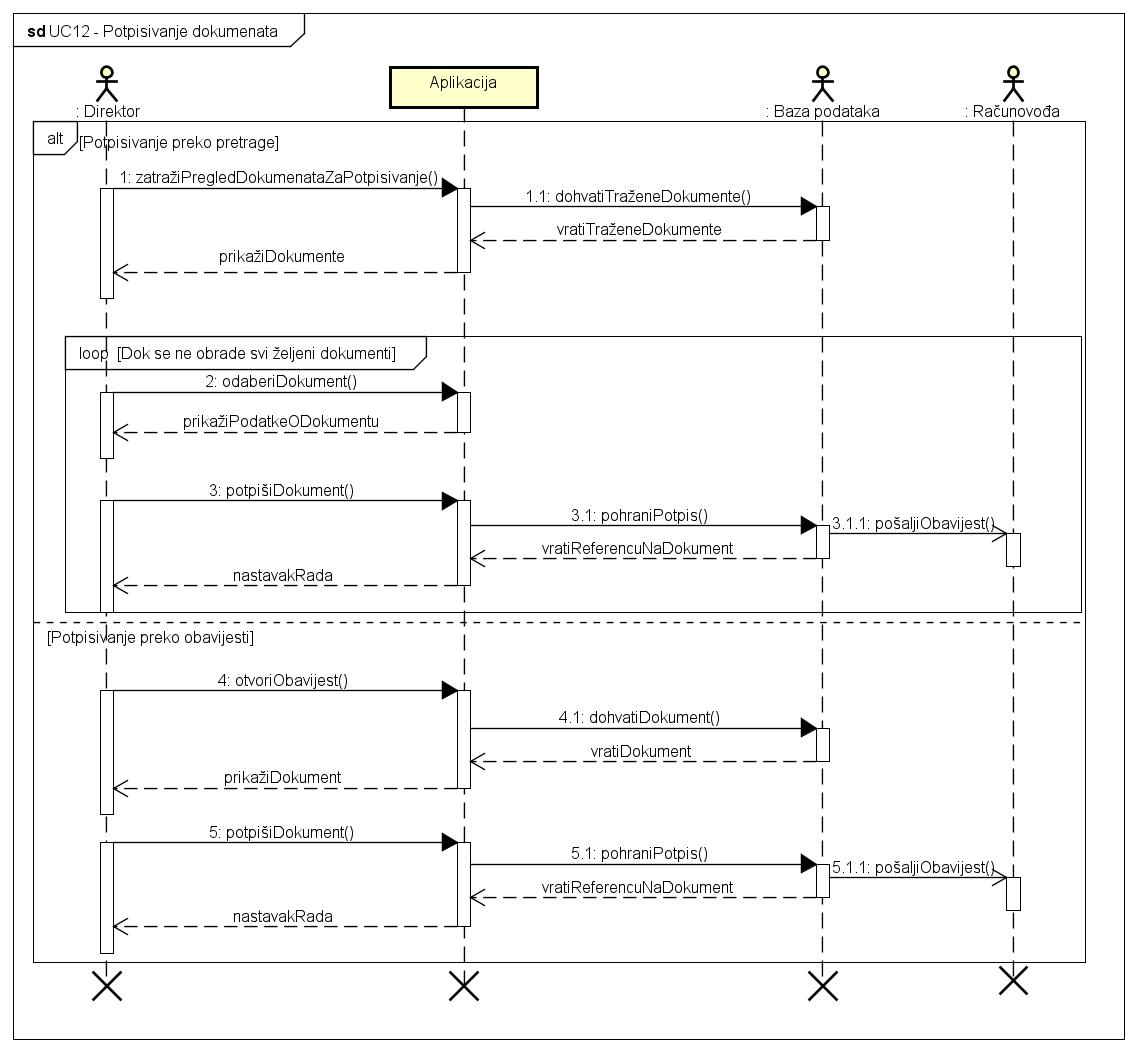
\includegraphics[scale=0.35]{slike/UC12 - Potpisivanje dokumenata} %veličina slike u odnosu na originalnu datoteku i pozicija slike
					\centering
					\caption{ Sekvencijalni dijagram, UC12}
					\label{fig:promjene}
				\end{figure}
				\eject
	
		\section{Ostali zahtjevi}
		\begin{packed_item}
			\item{Aplikacija mora omogućiti primanje obavijesti i kada korisnik nema otvorenu instancu aplikacije}
			\item{Izvođenje OCR algoritma ne smije trajati duže od nekoliko sekundi}
			\item{Sustav mora podržavati rad od 50 do 100 korisnika u stvarnom vremenu}
			\item{Aplikacija za detektiranje prisutnosti dokumenta mora koristiti detekciju rubova}
			\item{Sustav za praćenje broja skeniranih dokumenata koristi pomoćnu strukturu podataka kako bi se smanjio broj upita u bazu podataka}
			\item{Sustav za prikaz velikog broja dokumenata mora koristi paginaciju \textit{(eng. pagination)}}
			\item{Aplikacija prilikom ponovnog otvaranja mora pamtiti zadnje prijavljenog korisnika}
			\item{Aplikacija prilikom pregleda dokumenata mora omogućiti naprednije filtriranje i sortiranje}
			\item{Aplikacija mora podržavati prijavu različitih korisnika na istom uređaju}
		\end{packed_item}
			
			 
			 
			 
	
	\chapter{Arhitektura i dizajn sustava}
	
	\justify{Arhitektura se može podijeliti na sljedeće podsustave:}
	\begin{itemize}
		\item Mobilni uređaj
		\item Mobilna aplikacija
		\item Baza podataka	
	\end{itemize}

	\begin{figure}[h]
		\centering
		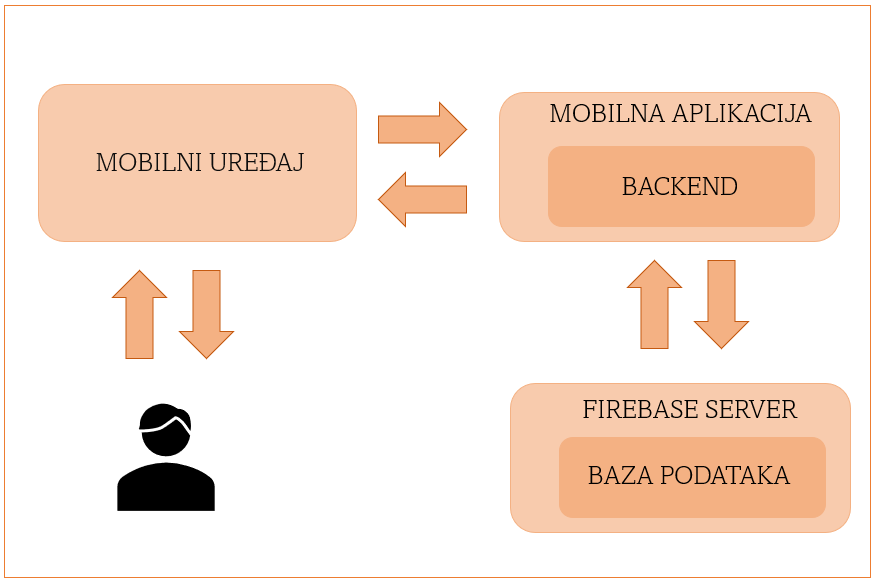
\includegraphics[width=\textwidth]{Arhitektura.png}
		\caption{Arhitektura sustava}
	\end{figure}

	\justify{\textbf{Mobilni (Android) uređaj} je uređaj koji korisniku omogućuje pokretanje Android mobilne aplikacije. Aplikacija je napisana u kodu te nakon toga uređaj taj kod interpretira i prikazuje ga korisniku kao grafičko sučelje. Pomoću uređaja
	korisnik ineraktira s aplikacijom i preko nje šalje upite bazi podataka.}

	\justify{\textbf{Mobilna aplikacija} je glavni dio arhitekture. Korisnik istu koristi kako bi obradio svoje zahtjeve. Ona se sastoji od \textit{Frontend} i \textit{Backend} dijela te pomoću \textit{Backenda} komunicira s bazom podataka, čitajući ili pišući podatke u nju. Nakon toga se korisniku preko \textit{Frontend} dijela
	prikazuju potrebni podaci.}

	Programski jezik koji smo koristili za izradu naše mobilne je Kotlin, koji je Google 2019. proglasio kao preferirani jezik izrade Android aplikacija. Razvojno okruženje
	s najboljom podrškom za izradu takvih aplikacija je Android Studio, koji smo i mi upotrebljavali. Jedan dio \textit{Backend} programskog koda napisan je u JavaScript programskom jeziku, 
	u Node.js okruženju. Arhitektura sustava se temelji na MVVM (Model-View-Viewmodel) konceptu, koji je dio svake Android aplikacije.

	Odlika MVVM-a je što pomaže organizirati kod i podijeliti program u manje dijelove kako bi razvoj, ažuriranje i ponovna upotreba koda bila jednostavnija i brža.
	MVVM se sastoji od:
	\begin{itemize}
		\item \textbf{Model} - odnosi se ili na model domene, koji predstavlja sadržaj stvarnog stanja (objektno orijentirani pristup), ili na sloj pristupa podacima, koji predstavlja sadržaj.
		\item \textbf{View} - struktura, raspored i izgled onoga što korisnik vidi na zaslonu. Prikazuje model i 
		prima interakciju korisnika s prikazom (klikovi mišem, unos tipkovnice, dodirivanja zaslona, itd.).
		\item \textbf{Viewmodel} - nalazi se između Viewa i Modela. Ovdje su smještene kontrole za interakciju s Viewom, dok se \textit{binding} koristi za povezivanje elemenata korisničkog sučelja
		 u Viewu s kontrolama u ViewModelu.
	\end{itemize}
	
				
		\section{Baza podataka}
			
		\justifying{Za potrebe našeg sustava koristit ćemo nerelacijsku bazu podataka (NoSQL) ugrađenu u Firebase alat koji olakšava rad s podatcima. Firebase nudi nekoliko vrsta baza, a mi smo izabrali Firestore verziju. Baza se sastoji od nekoliko kolekcija koja se definira imenom i skupom dokumenata, a svaki dokument ima svoje atribute. Atributi se sastoje od imena, tipa podataka i samog podatka. Temelje se na modelu ključ-vrijednost. Kako svaki dokument unutar kolekcije može imati različite atribute, važno je održati konzistentnost podataka, baza mora biti dosljedna i to se postiže kreiranjem modela unutar aplikacije. Na taj način će svi dokumenti unutar kolekcije imati iste atribute.
		Baza se sastoji od sljedećih kolekcija: 
		}
		\begin{itemize}
			\item documentArchive
			\item documentStatus
			\item documentByUser
			\item documents 
			\item users
			\item tokens
		\end{itemize}
		
			\subsection{Opis tablica}
			

			\justify{\textit{\textbf{Napomena:} Iz razloga što se u službenoj Firebase dokumentaciji koriste izrazi collection i document te zato što se naša aplikacija bavi skeniranjem dokumenata, može doći do zabune kad je koji izraz za dokument upotrijebljen (Firebaseov ili iz aplikacije). Stoga će se u daljnjem tekstu za izraz koji se odnosi na fizičke (skenirane) dokumente koristiti riječ \textbf{dokument}, a za Firebaseov član kolekcije riječ \textbf{document}.}}

			\justify{\textbf{documentArchive}   Ova kolekcija sadrži informaciju o arhiviranju dokumenata. Dokumentu koji je arhiviran, tj. spremljen u bazu, se automatski generira identifikator te \textit{documenti} u \textit{documentArchive} kolekciji dobivaju iste te identifikatore, kako bi se znalo za koji skenirani dokument sadrži podatke. Kolekcija se sastoji od atributa \textit{archiveId} i \textit{archivedOn}, koji govori vrijeme kreiranja arhive. Svakom \textit{documentu} iz kolekcije \textit{documents} pripada jedan \textit{document} iz kolekcije \textit{documentArchive}.}
			
				\begin{longtblr}[
					label=none,
					entry=none
					]{
						width = \textwidth,
						colspec={|X[6,l]|X[6, l]|X[20, l]|}, 
						rowhead = 1,
					} %definicija širine tablice, širine stupaca, poravnanje i broja redaka naslova tablice
					\hline \multicolumn{3}{|c|}{\textbf{documentArchive}}	 \\ \hline[3pt]
					\SetCell{LightGreen}documentId & string	&  	Jedinstveni identifikator arhive. Jednak id-u dokumenta koji je arhiviran\\ \hline
					archiveId	& string &   	\\ \hline 
					archivedOn  & timestamp & datum i vrijeme arhiviranja dokumenta   \\ \hline
				\end{longtblr}


			\justify{\textbf{documentStatus}  Ova se kolekcija sastoji od nekoliko atributa vezanih za status dokumenta. Sadrži atribute \textit{archived, revised, scannedProperly, toBeSigned, signed}. Primjerice, nakon što se dokument uspješno skenira, vrijednosti \textit{archived, scannedProperly} i \textit{toBeSigned} se postavljaju na \textit{true}. U slučaju da u aplikaciji treba filtrirati dokumente koji zadovoljavaju jedan ili više statusa, ova kolekcija dolazi u uporabu. Za svaki \textit{document} iz kolekcije \textit{documents} postoji jedan   \textit{document} iz ove kolekcije, s istim identifikatorom.}
				
				\begin{longtblr}[
					label=none,
					entry=none
					]{
						width = \textwidth,
						colspec={|X[10,l]|X[6, l]|X[20, l]|}, 
						rowhead = 1,
					} %definicija širine tablice, širine stupaca, poravnanje i broja redaka naslova tablice
					\hline \multicolumn{3}{|c|}{\textbf{documentStatus}}	 \\ \hline[3pt]
					\SetCell{LightBlue}documentId & string	&  	Jedinstveni identifikator. Jednak id-u dokumenta koji je skeniran\\ \hline
					archived	& boolean &  oznaka je li dokument arhiviran 	\\ \hline 
					revised  & boolean & oznaka je li dokument reviziran   \\ \hline
					scannedProperly  & boolean & oznaka je li dokument pravilno skeniran   \\ \hline
					signed  & boolean & oznaka je li dokument potpisan   \\ \hline
					toBeSigned  & boolean & oznaka je li dokument poslan na slanje   \\ \hline
					
				\end{longtblr}

				\justify{\textbf{documentByUser}  Kolekcija koja informira o detaljnijim podacima dokumenta, tj. prikazuje koji je \textit{user} napravio koji korak u protoku dokumenta kroz aplikaciju. Sadrži atribute \textit{archivedBy, revisedBy, sentToSignBy, signedBy}. U polju svakog od atributa nalazi se  id nekog \textit{usera}. Za svaki \textit{document} iz kolekcije \textit{documents} postoji jedan   \textit{document} iz ove kolekcije, s istim identifikatorom.				
				\begin{longtblr}[
					label=none,
					entry=none
					]{
						width = \textwidth,
						colspec={|X[10,l]|X[6, l]|X[20, l]|}, 
						rowhead = 1,
					} %definicija širine tablice, širine stupaca, poravnanje i broja redaka naslova tablice
					\hline \multicolumn{3}{|c|}{\textbf{documentByUser}}	 \\ \hline[3pt]
					\SetCell{LightBlue}documentId & string	&  	Jedinstveni identifikator. Jednak id-u dokumenta koji je skeniran\\ \hline
					archivedBy	& string &  id usera koji je arhivirao dokument 	\\ \hline 
					revisedBy  & boolean & id usera koji je revizirao dokument   \\ \hline
					toBeSignBy  & boolean & id usera koji je dokument poslao na potpisivanje \\ \hline
					signedBy  & boolean & id usera koji je potpisao dokument  \\ \hline
				\end{longtblr}
			

			\justify{\textbf{documents}  Kolekcija koja sadrži informacije o skeniranim dokumentima. Postoji nekoliko specijalizacija dokumenta, a to su \textbf{Račun}, \textbf{Ponuda} i \textbf{Interni dokument}. Dokumenti sadrže zajednički skup atributa, \textit{createdOn}, \textit{type}, \textit{user}, \textit{label} te svaka od specijalizacija ima svoje zasebne atribute. Svakom dokumentu se može pridružiti jedan \textit{document} iz kolekcija \textit{documentArchive}, \textit{documentStatus} i \textit{users}. Identifikator pojedinog \textit{usera} se u ovoj kolekciji sprema pod atribut \textit{user}.}
				
				\begin{longtblr}[
					label=none,
					entry=none
					]{
						width = \textwidth,
						colspec={|X[10,l]|X[6, l]|X[20, l]|}, 
						rowhead = 1,
					} %definicija širine tablice, širine stupaca, poravnanje i broja redaka naslova tablice
					\hline \multicolumn{3}{|c|}{\textbf{documents}}	 \\ \hline[3pt]
					\SetCell{LightGreen}documentId & string	&  	Jedinstveni identifikator skeniranog dokumenta\\ \hline
					createdOn  & timestamp & datum i vrijeme kreiranja dokumenta   \\ \hline
					label  & string & oznaka s dokumenta   \\ \hline
					type  & string & tip dokumenta: Račun, Ponuda, Interni dokument   \\ \hline
					user  & string & ID korisnika koji je obavio skeniranje   \\ \hline
					clientName	& string &  ime i prezime klijenta s Računa	\\ \hline 
					items  & map of numbers & artikli s Računa ili Ponude   \\ \hline
					totalPrice  & number & ukupna cijena artikala s Računa ili Ponude   \\ \hline
					content  & string & sadržaj Internog dokumenta   \\ \hline
				\end{longtblr}

			\justify{\textbf{users}  Ova kolekcija sadrži informacije o korisnicima aplikacije koji su registrirani. Pri prvoj uporabi aplikacije svaki korisnik mora proći registraciju. U kolekciji se pohranjuju korisnikov email, ime, prezime i uloga. Korisnik može biti Direktor, Računovođa, Revizor ili Zaposlenik. Svoju ulogu korisnik odabire pri registraciji. Svaki korisnik ima svoj ID i on se sprema u kolekciju \textit{documents}, kako bi se znalo koji korisnik je skenirao koji dokument.}
				
				\begin{longtblr}[
					label=none,
					entry=none
					]{
						width = \textwidth,
						colspec={|X[6,l]|X[6, l]|X[20, l]|}, 
						rowhead = 1,
					} %definicija širine tablice, širine stupaca, poravnanje i broja redaka naslova tablice
					\hline \multicolumn{3}{|c|}{\textbf{users}}	 \\ \hline[3pt]
					\SetCell{LightGreen}documentId & string	&  	Jedinstveni identifikator registriranog korisnika\\ \hline
					email  & string & email adresa korisnika   \\ \hline
					firstName  & string & ime korisnika  \\ \hline
					lastName  & string & prezime korisnika   \\ \hline
					role  & string & uloga korisnika   \\ \hline
					specialization  & string & opcionalna specijalizacija Računovođe   \\ \hline
					
				\end{longtblr}	

			\justify{\textbf{tokens} Kolekcija s \textit{Firebase Cloud Messaging} tokenima. Ona omogućava slanje notifikacijama onim tokenima koji su u tom trenutku aktivni ili zadovoljavaju određene uvjete. Sastoji se od samo jednog atributa, \textit{token}, a jedinstveni identifikator tokena je jednak identifikatoru jednom \textit{documentu} iz kolekcije \textit{users}.}

				\begin{longtblr}[
					label=none,
					entry=none
					]{
						width = \textwidth,
						colspec={|X[6,l]|X[6, l]|X[20, l]|}, 
						rowhead = 1,
					} %definicija širine tablice, širine stupaca, poravnanje i broja redaka naslova tablice
					\hline \multicolumn{3}{|c|}{\textbf{tokens}}	 \\ \hline[3pt]
					\SetCell{LightBlue}documentId & string	&  	Jedinstveni identifikator tokena. Jednak id-u usera kojem pripada.\\ \hline
					token & string & Identifikator dodijeljen od \textit{Firebase Cloud Messaginga} \\ \hline
					
				\end{longtblr}	
			
			\subsection{Dijagram baze podataka}
			\begin{figure}[h]
				\centering
				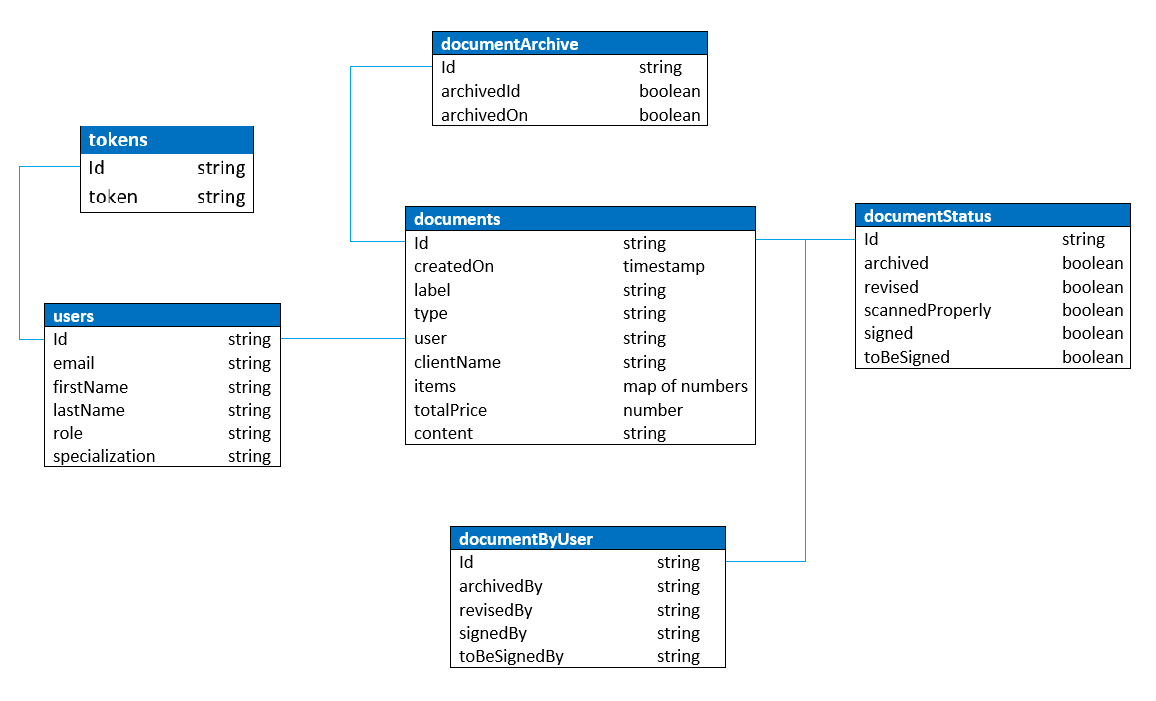
\includegraphics[width=\textwidth]{dijagramBaze.png}
				\caption{Dijagram baze podataka sustava}
			\end{figure}
			
			\eject
			
			
		\section{Dijagram razreda}
		
			\justify{Na slikama 4.3., 4.4., 4.5., 4.6. prikazani su razredi koji pripadaju MVVM arhitekturi. Zbog lakše organizacije, razredi su podijeljeni prema arhitekturi, kako bi se smanjila prenapučenost unutar dijagrama. Iz naziva i tipova podataka može se zaključiti vrsta ovisnosti između razreda.}\\
			
				
			\justify{Razredi prikazani na slici 4.3. nasljeđuju Activity i Fragment razred. Metode implementirane u tim razredima manipuliraju objektima dobivenim iz razreda sa slike 4.4. (ViewModel) te omogućuju prikaz podataka.}\\
			
			\begin{figure}[H]
				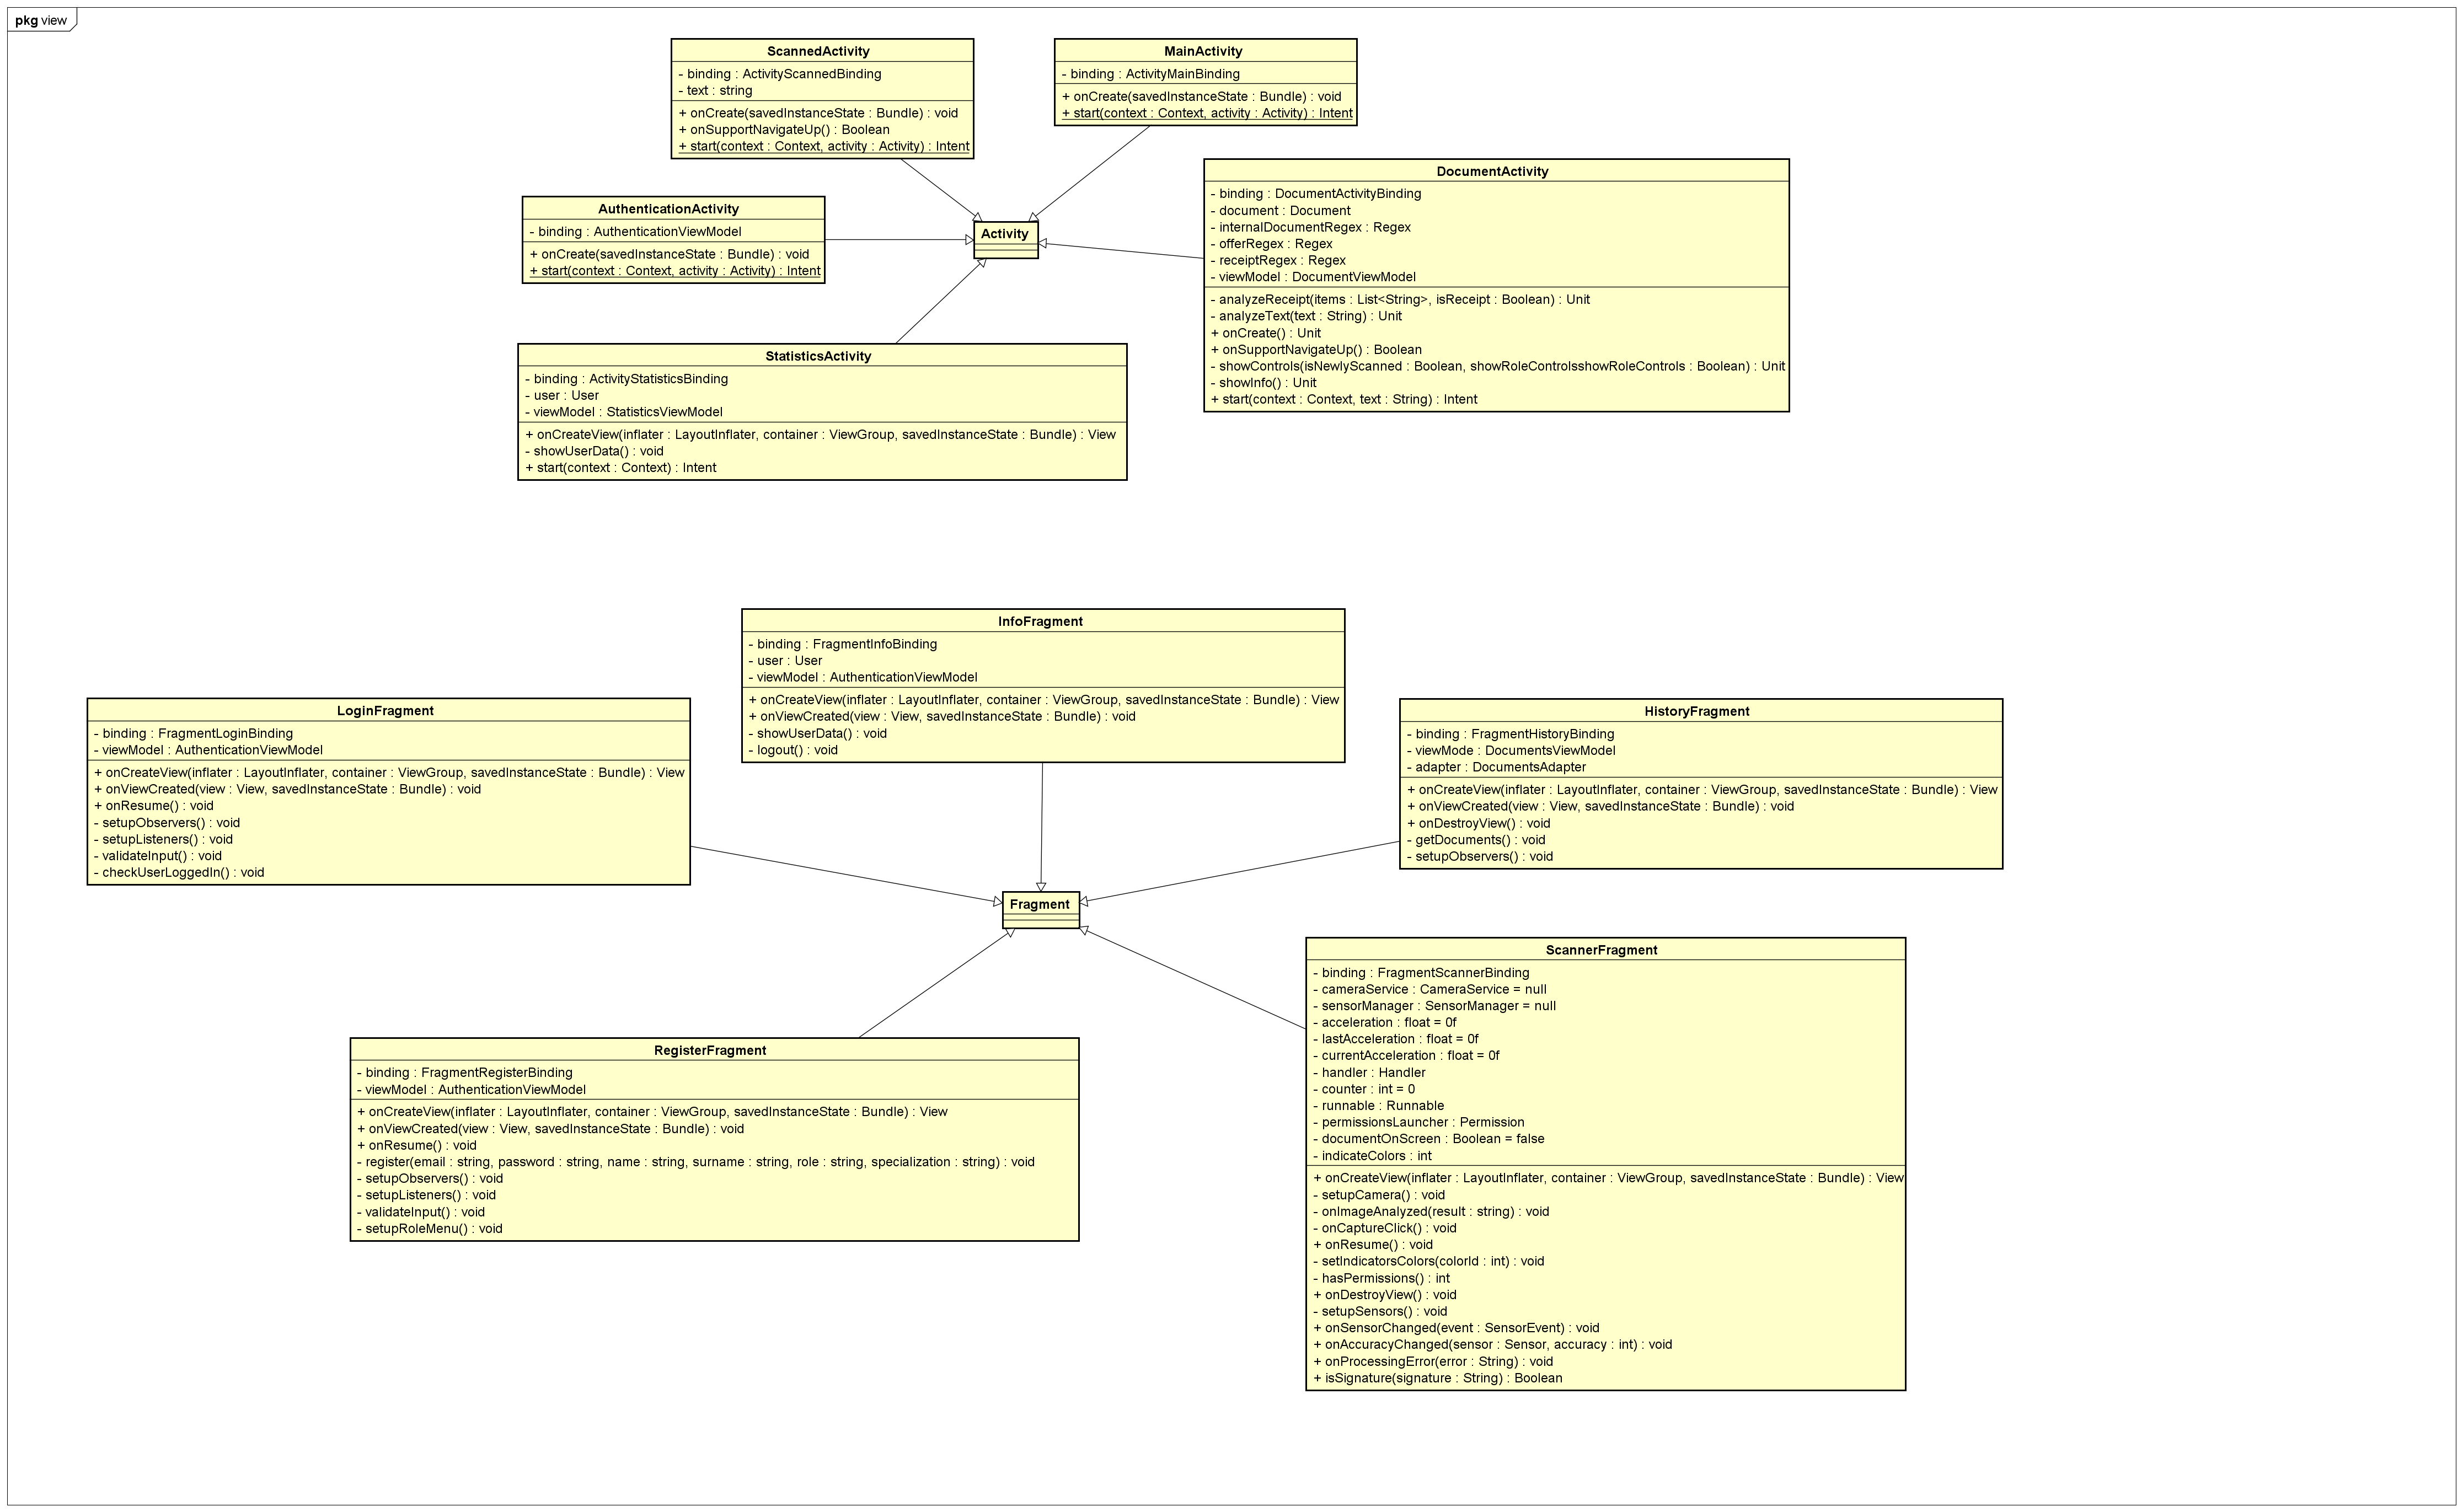
\includegraphics[width=\textwidth]{slike/Dijagram_razreda_view.png}
				\caption{Dijagram razreda - View.}
			\end{figure}
		
			\justify{Razredi DocumentsViewModel i AuthenticationViewModel uzimaju željene podatke preko razreda DocumentRepository i AuthenticationRepository, koji su direktno povezani s bazom podataka. AuthenticationRepository razred koristi se razredom AuthHelper kako bi prilikom registracije stvorio novog korisnika, a DocumentRepository koristi se razredom DocumentsHelper kako bi omogućio stvaranje dokumenata. Način na koji su povezani razredi iz view i viewModel dijela arhitekture prikazani su na slici 4.5.}\\
					
			\begin{figure}[H]
				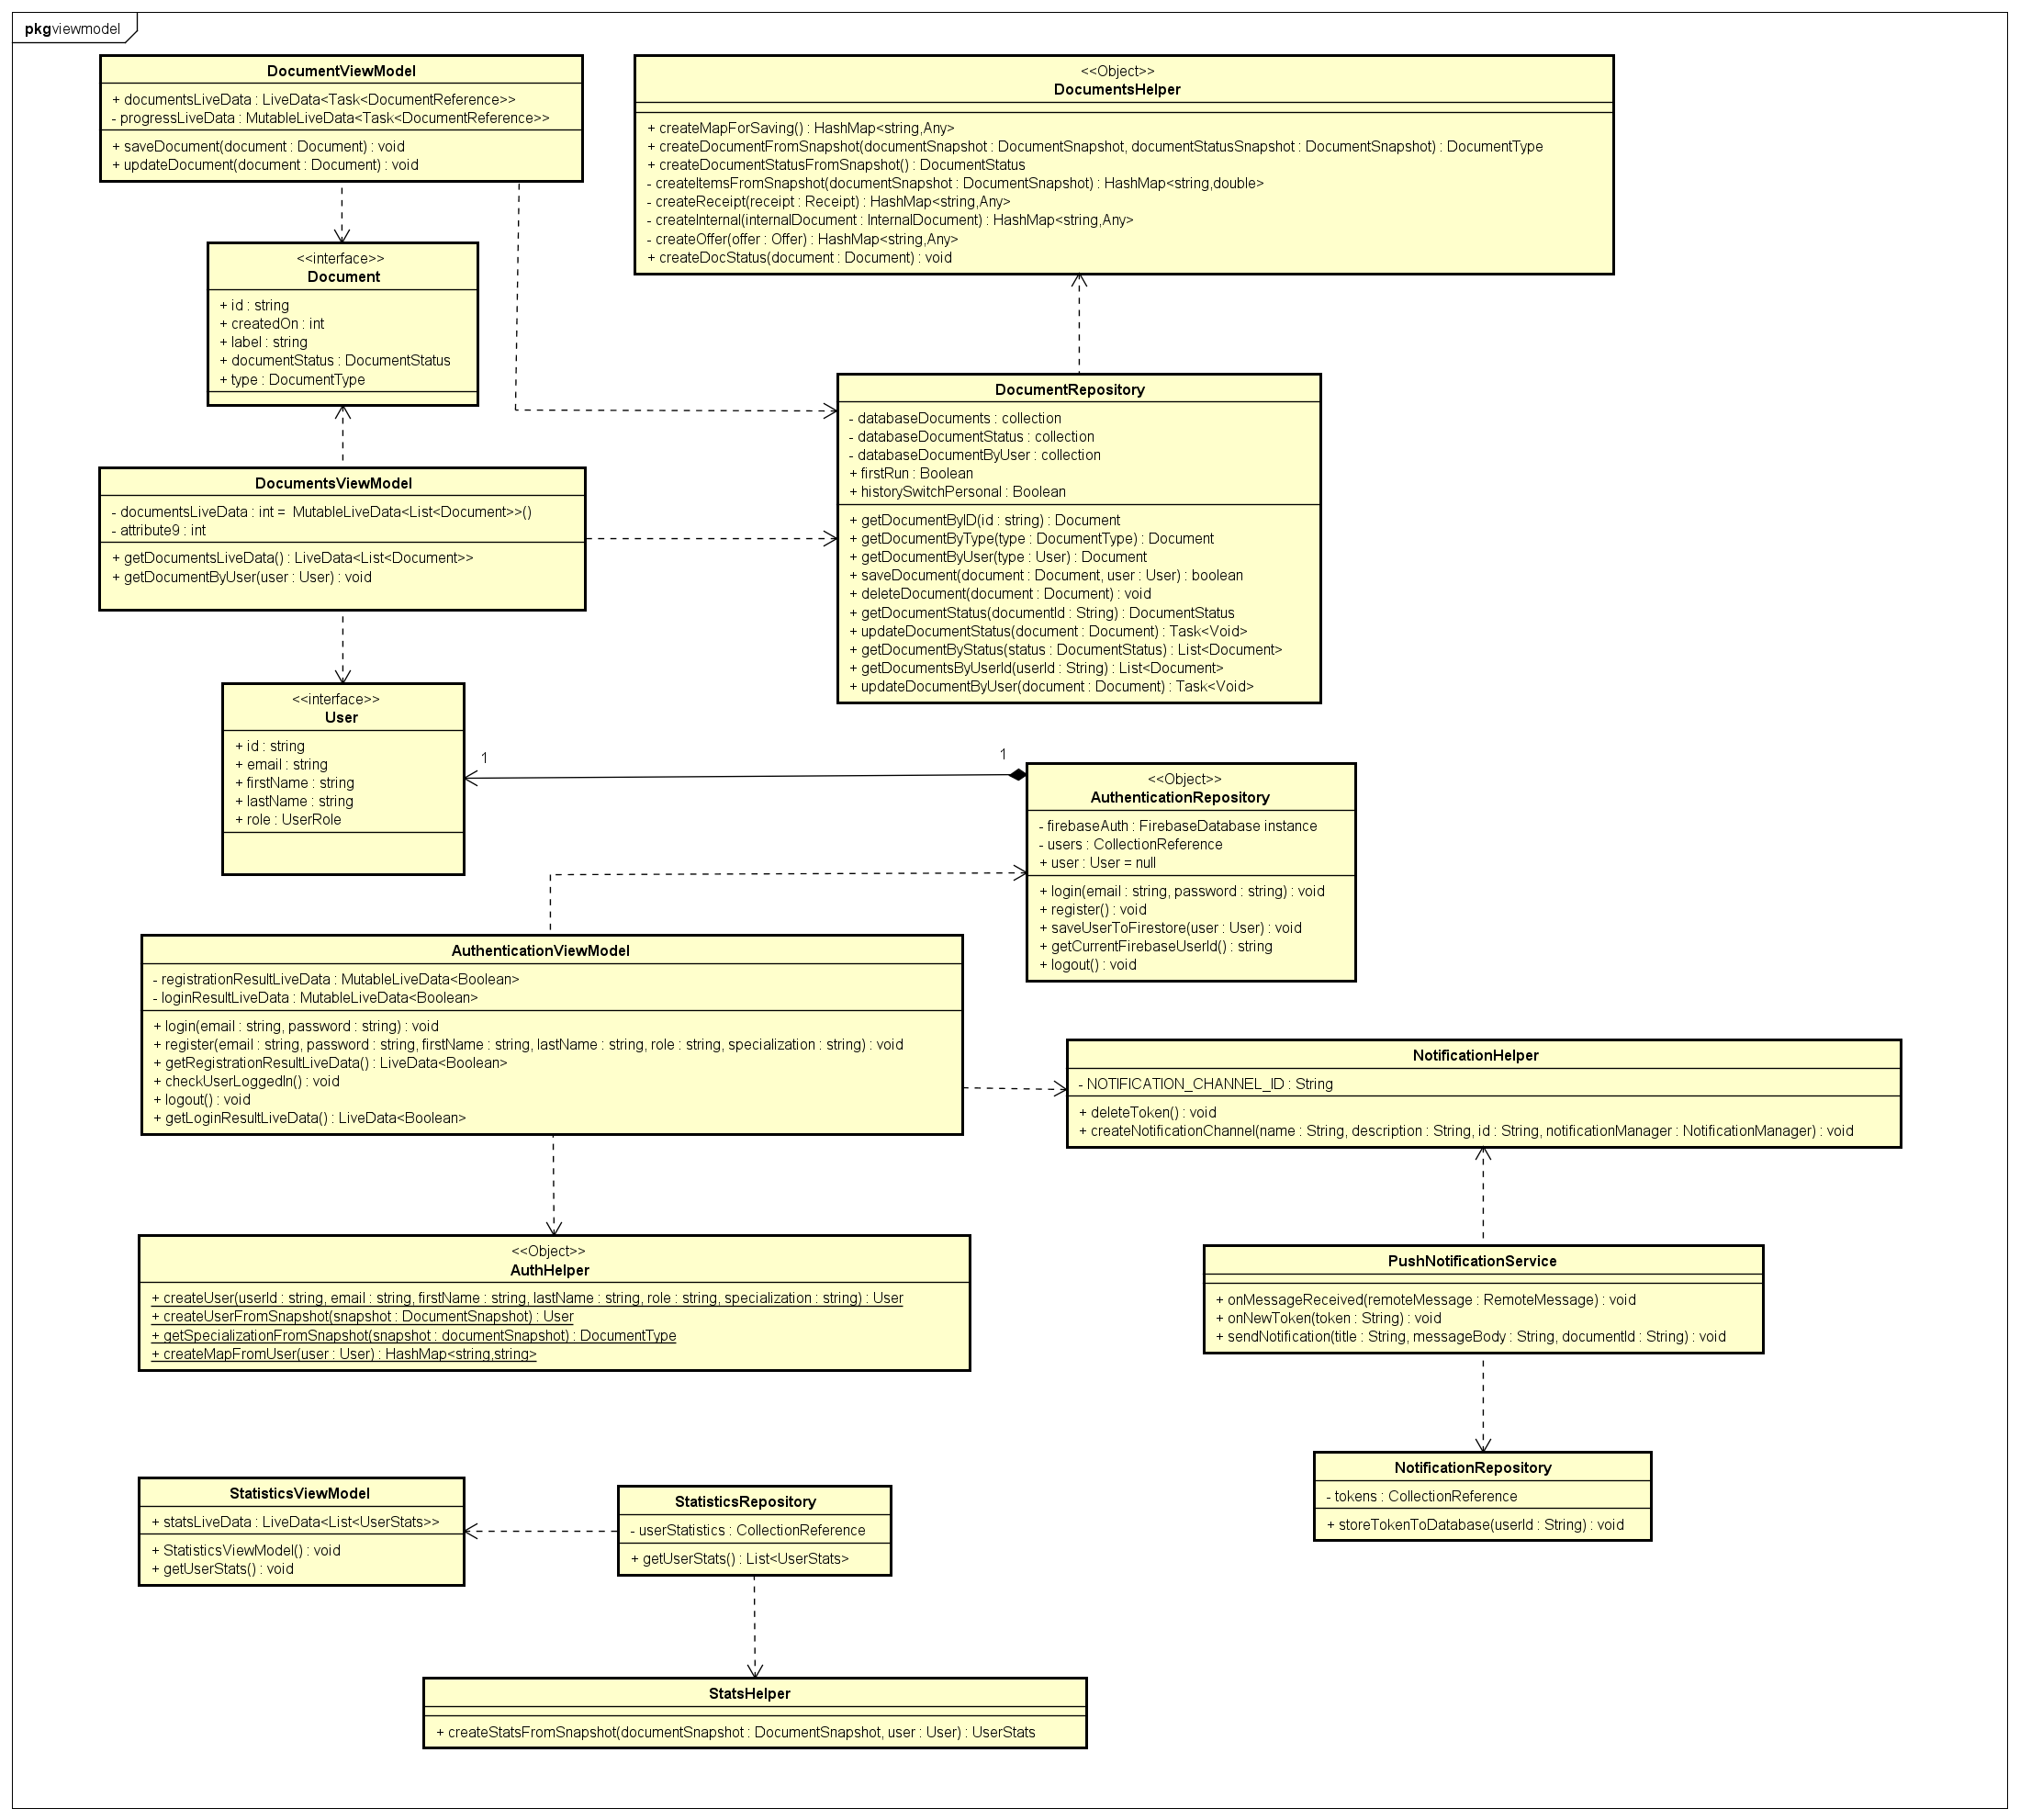
\includegraphics[width=\textwidth]{slike/Dijagram_razreda_viewModel.png}
				\caption{Dijagram razreda - ViewModel.}
			\end{figure}
		
			\begin{figure}[H]
				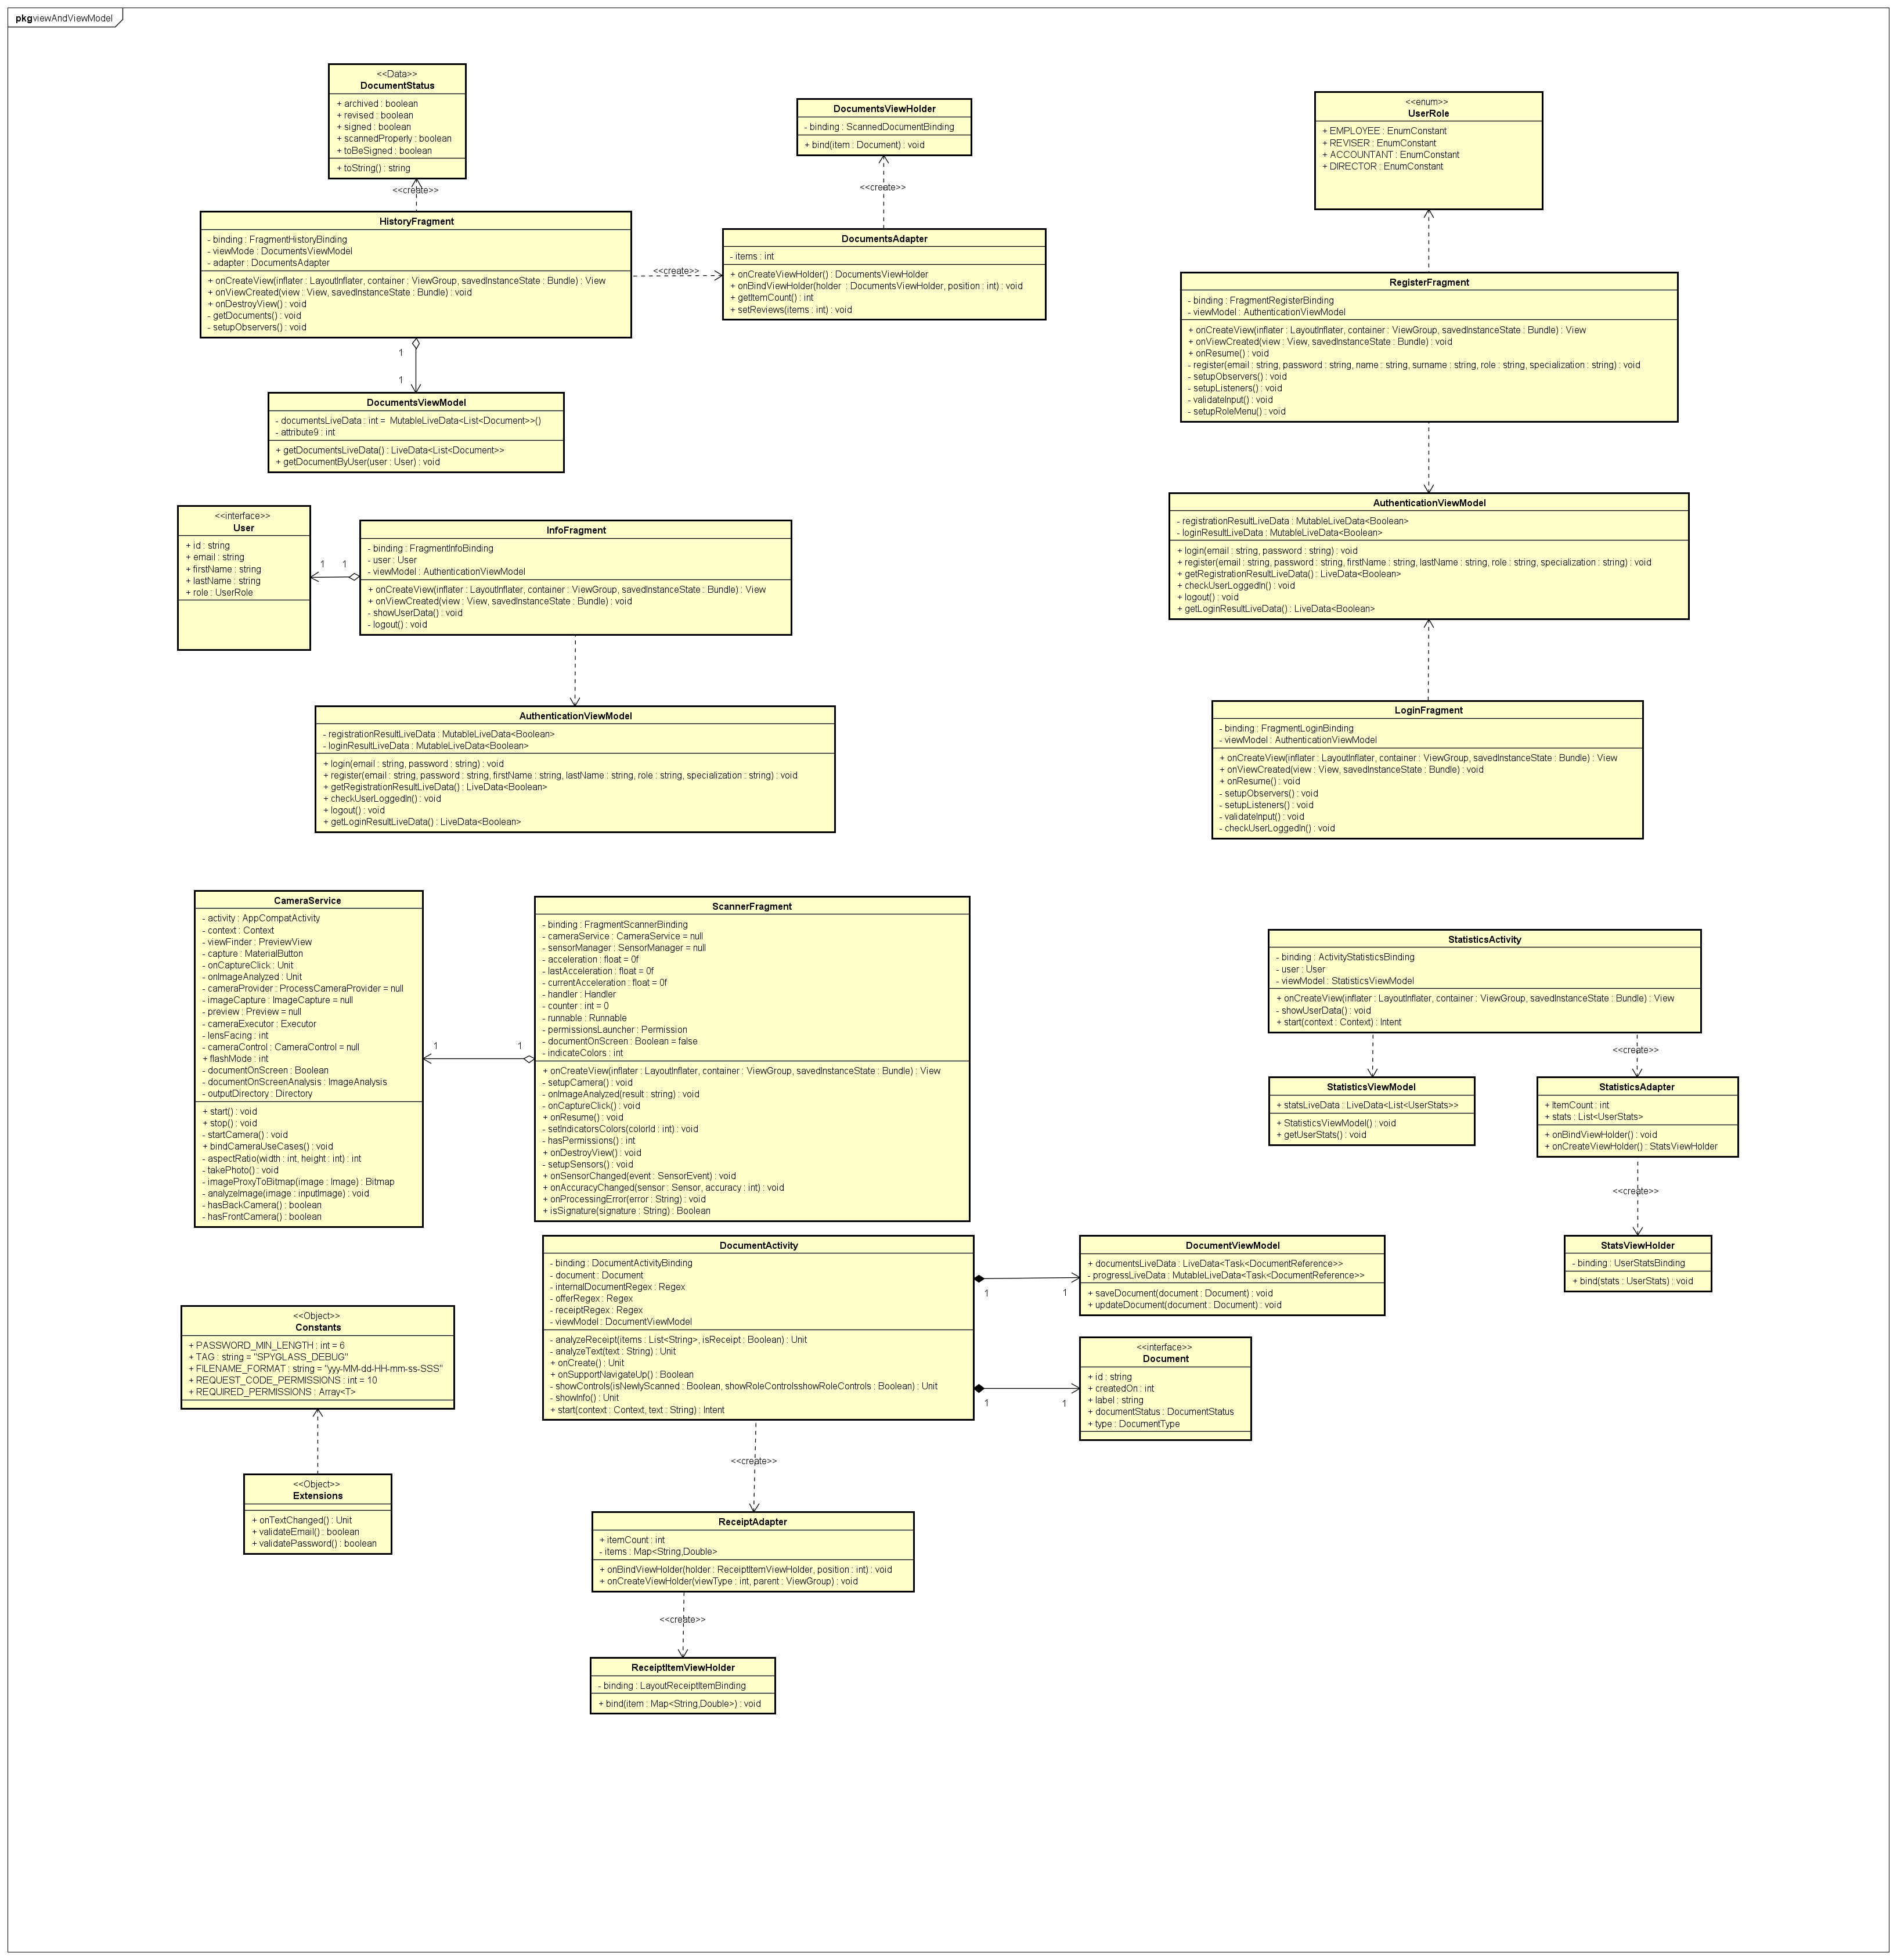
\includegraphics[width=\textwidth]{slike/Dijagram_razreda_viewAndViewModel.png}
				\caption{Dijagram razreda - View s ViewModelom.}
			\end{figure}
		
			\justify{Razredi koji su prikazani na slici 4.6. pripadaju model dijelu arhitekture. Razredi koji predstavljaju vrstu korisnika realiziraju sučelje User, a razredi koji predstavljaju vrstu dokumenta realiziraju sučelje Document.}
			
			\begin{figure}[H]
				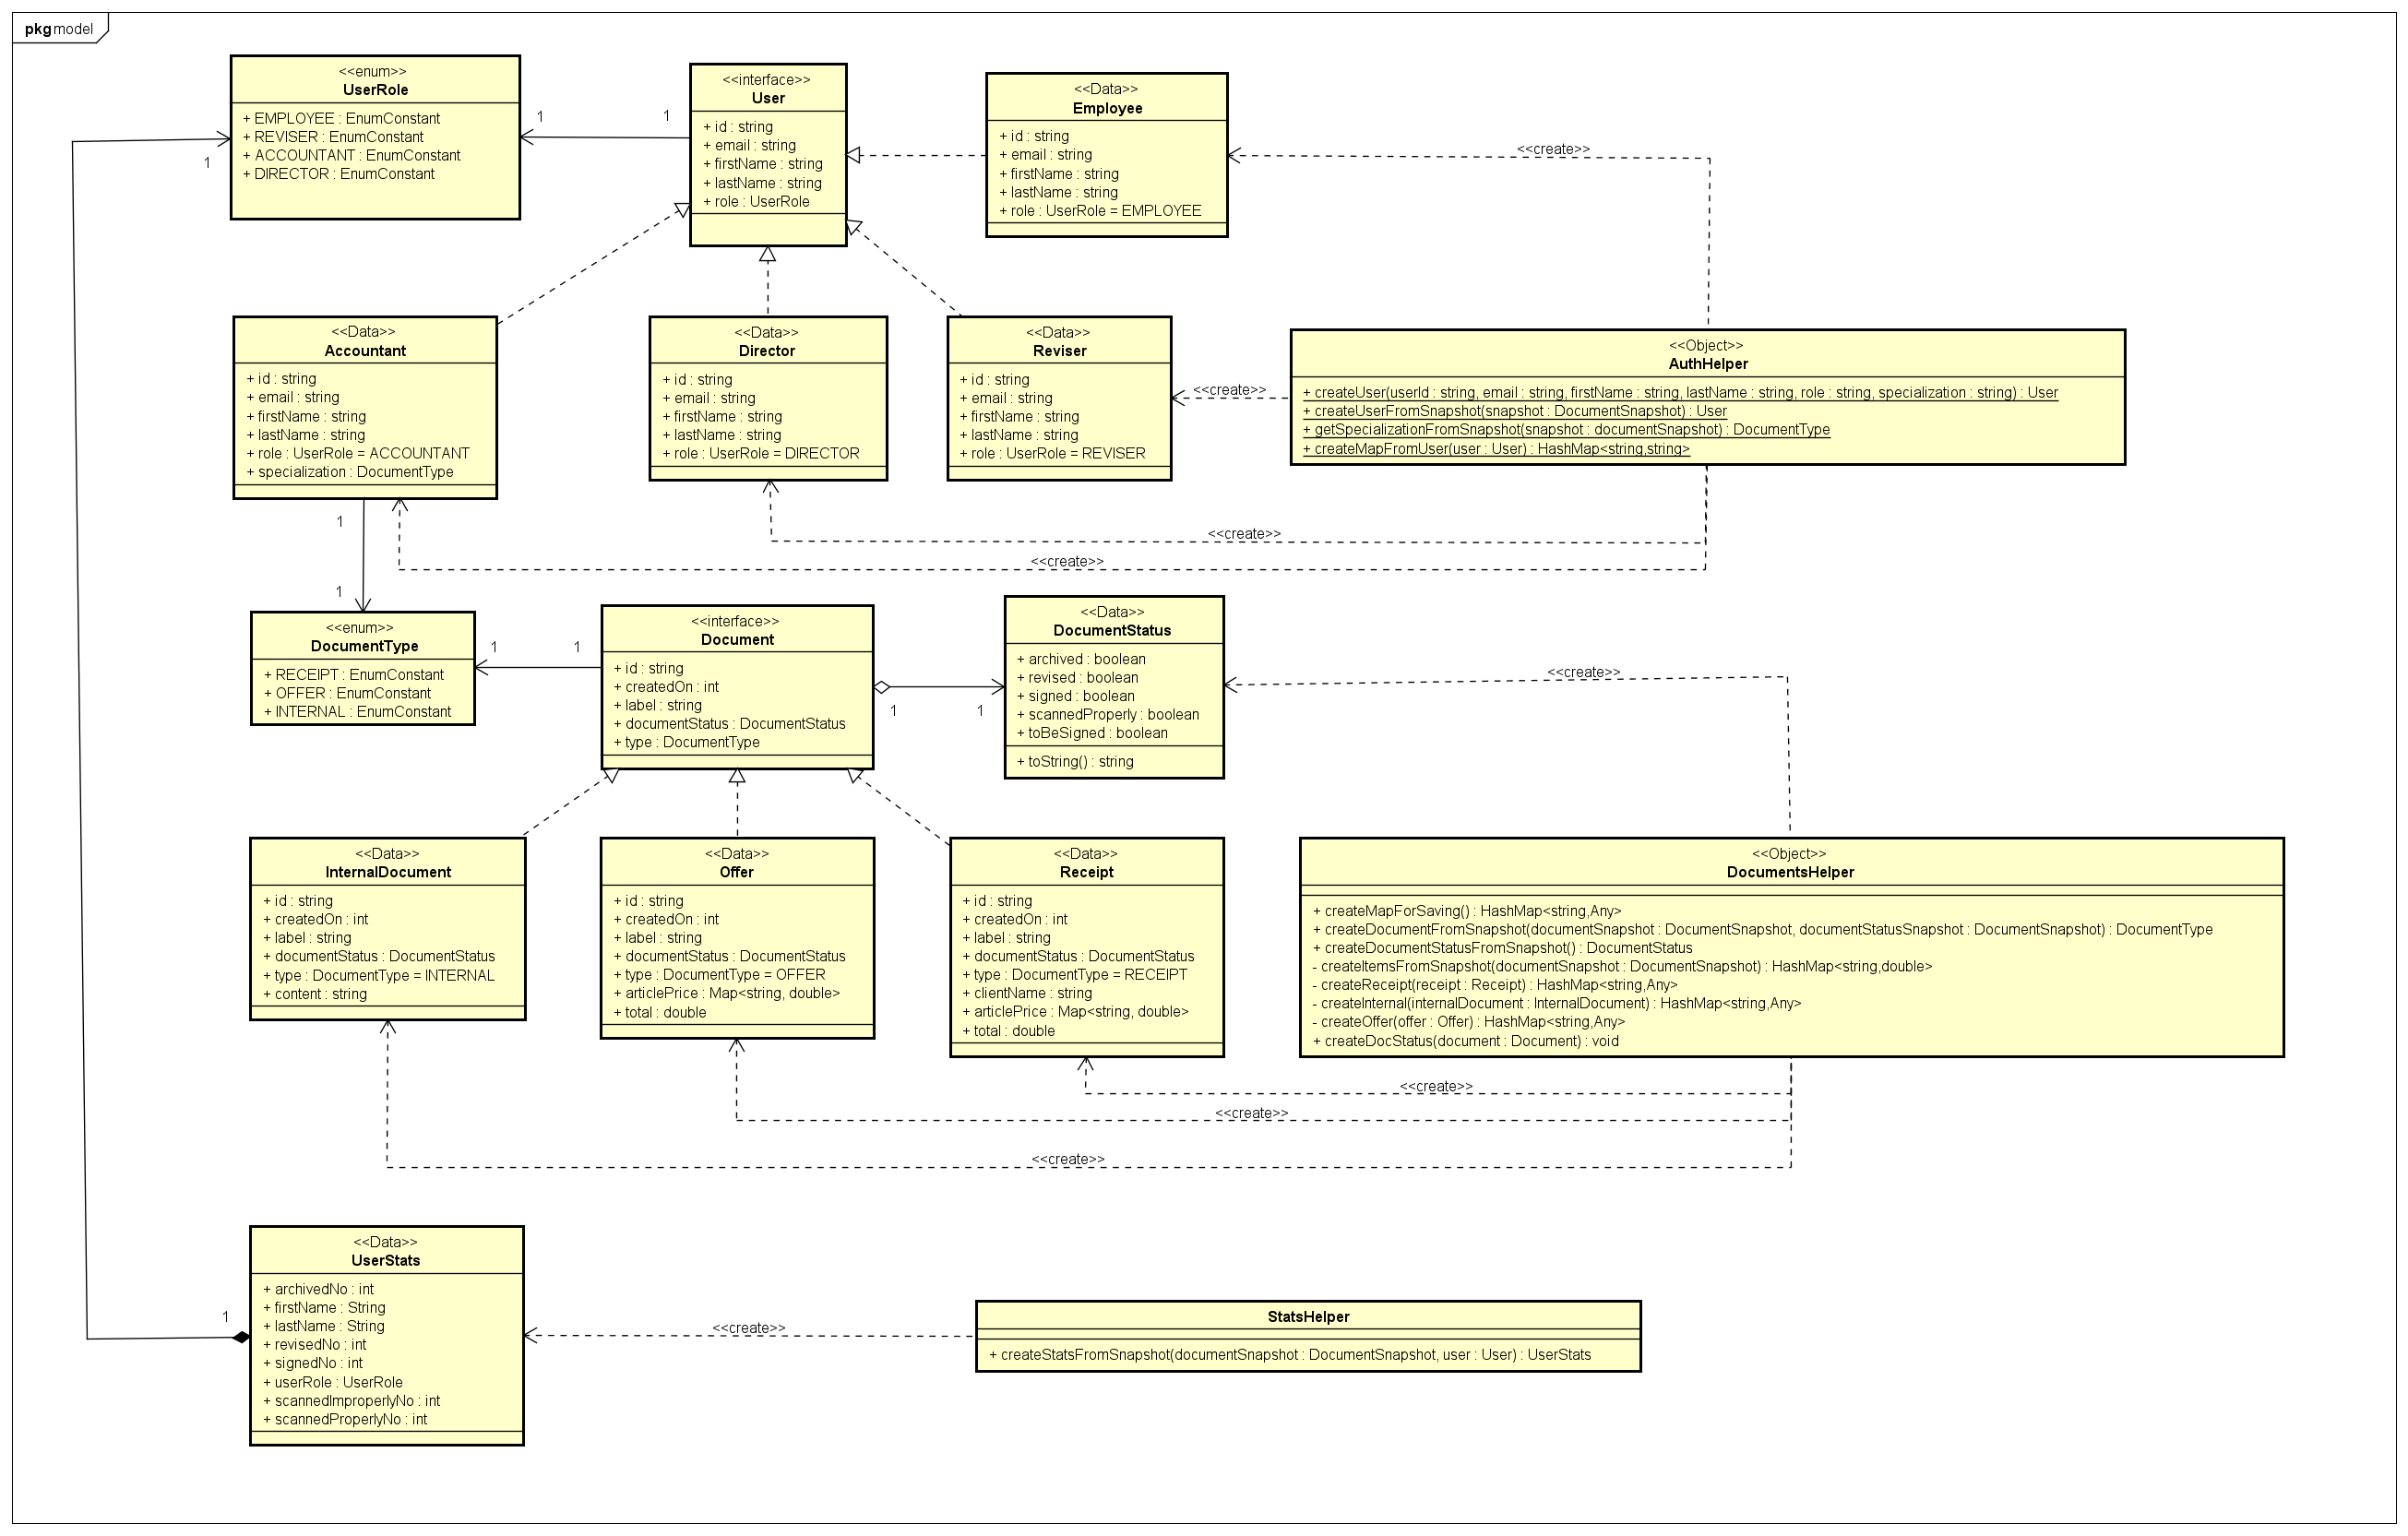
\includegraphics[width=\textwidth]{slike/Dijagram_razreda_model.png}
				\caption{Dijagram razreda - Model}
			\end{figure}
			
			
			\eject
		
		\section{Dijagram stanja}
			
				
			\justify{Dijagram stanja prikazuje stanja objekta te prijelaze iz jednog stanja u drugo temeljene na događajima. Na slici 4.7. prikazan je dijagram stanja za registriranog korisnika, koji može biti direktor, računovođa, revizor ili zaposlenik. Nakon prijave korisnik može skenirati dokument (nakon što akcelerometar i žiroskop to dopuste). Dodirom na gumb za skeniranje otvara se pregled skeniranog dokumenta. Ako korisnik nije zadovoljan skeniranim, ima opciju dodira na gumb \textit{Discard}, a u suprotnom gumb \textit{Save}. Bez obzira koji gumb je dodirnut, aplikacija vraća korisnika na karticu za skeniranje. Dodirom kartice \textit{History} korisniku se prikazuju osobni skenirani dokumenti. Postoji \textit{switch} koji kad se dodirne mijenja prikaz u dokumente koji su potrebni za obrađivanje (revizija, arhiviranje, potpisivanje – ovisno o tipu korisnika). U oba slučaja \textit{switcha} korisnik može dodirom na pojedini dokument vidjeti detalje dokumenta i obaviti akciju. Odlaskom na karticu \textit{Info} prijavljeni korisnik pregledava osobne podatke te ima mogućnost dodirnuti gumb za odjavu ili za prikaz statistike.}
			
			\begin{figure}[H]
				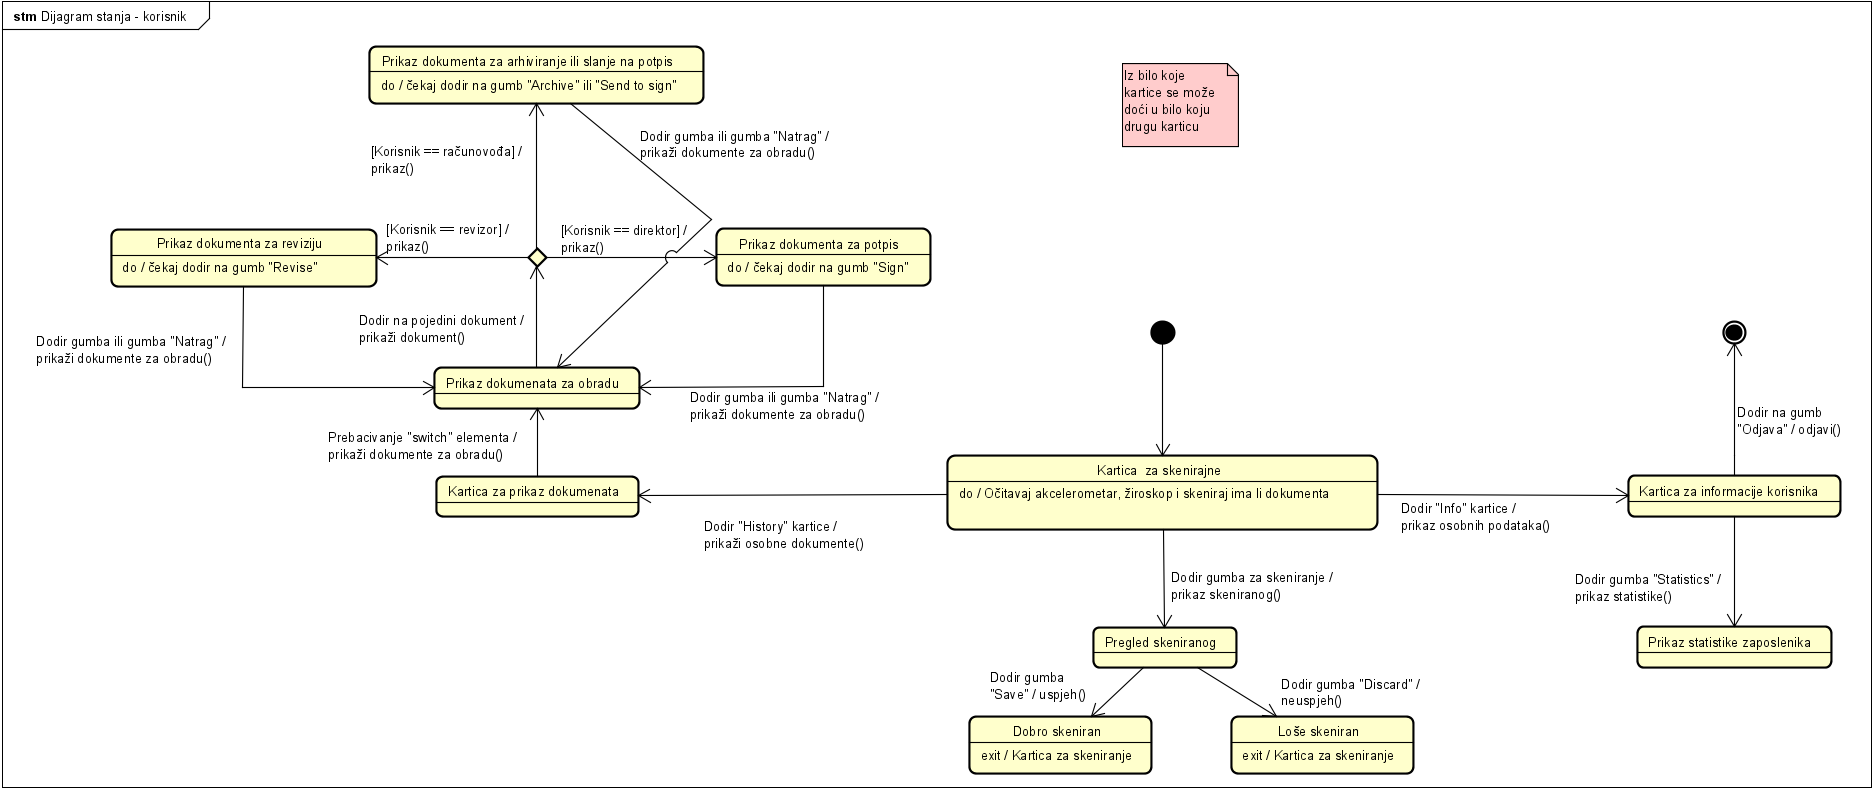
\includegraphics[width=\textwidth]{slike/Dijagram stanja.png}
				\caption{Dijagram stanja - Registrirani korisnik}
			\end{figure}
			
			\eject 
		
		\section{Dijagram aktivnosti}

			
			\justify{Dijagram aktivnosti primjenjuje se za opis modela toka upravljanja ili toka podataka. Na dijagramu aktivnosti prikazan je 
			proces skeniranja dokumenta. Pri modeliranju toka upravljanja svaki novi korak poduzima se nakon završenog prethodnog, osim koraka 
			\textit{Mirovanje od 5 s} i \textit{Detekcija dokumenta}, koji se odvijaju istovremeno. Korisnik se s korisničkim podacima prijavljuje u sustav, 
			skenira željeni dokument, nakon čega mu se prikazuje sažetak dokumenta. Korisnik zatim označava dokument kao dobro ili loše skeniran, 
			dokument se šalje u bazu podataka, te se zajedno s odabirom korisnika pohranjuje u bazu.}
			
			\begin{figure}[H]
				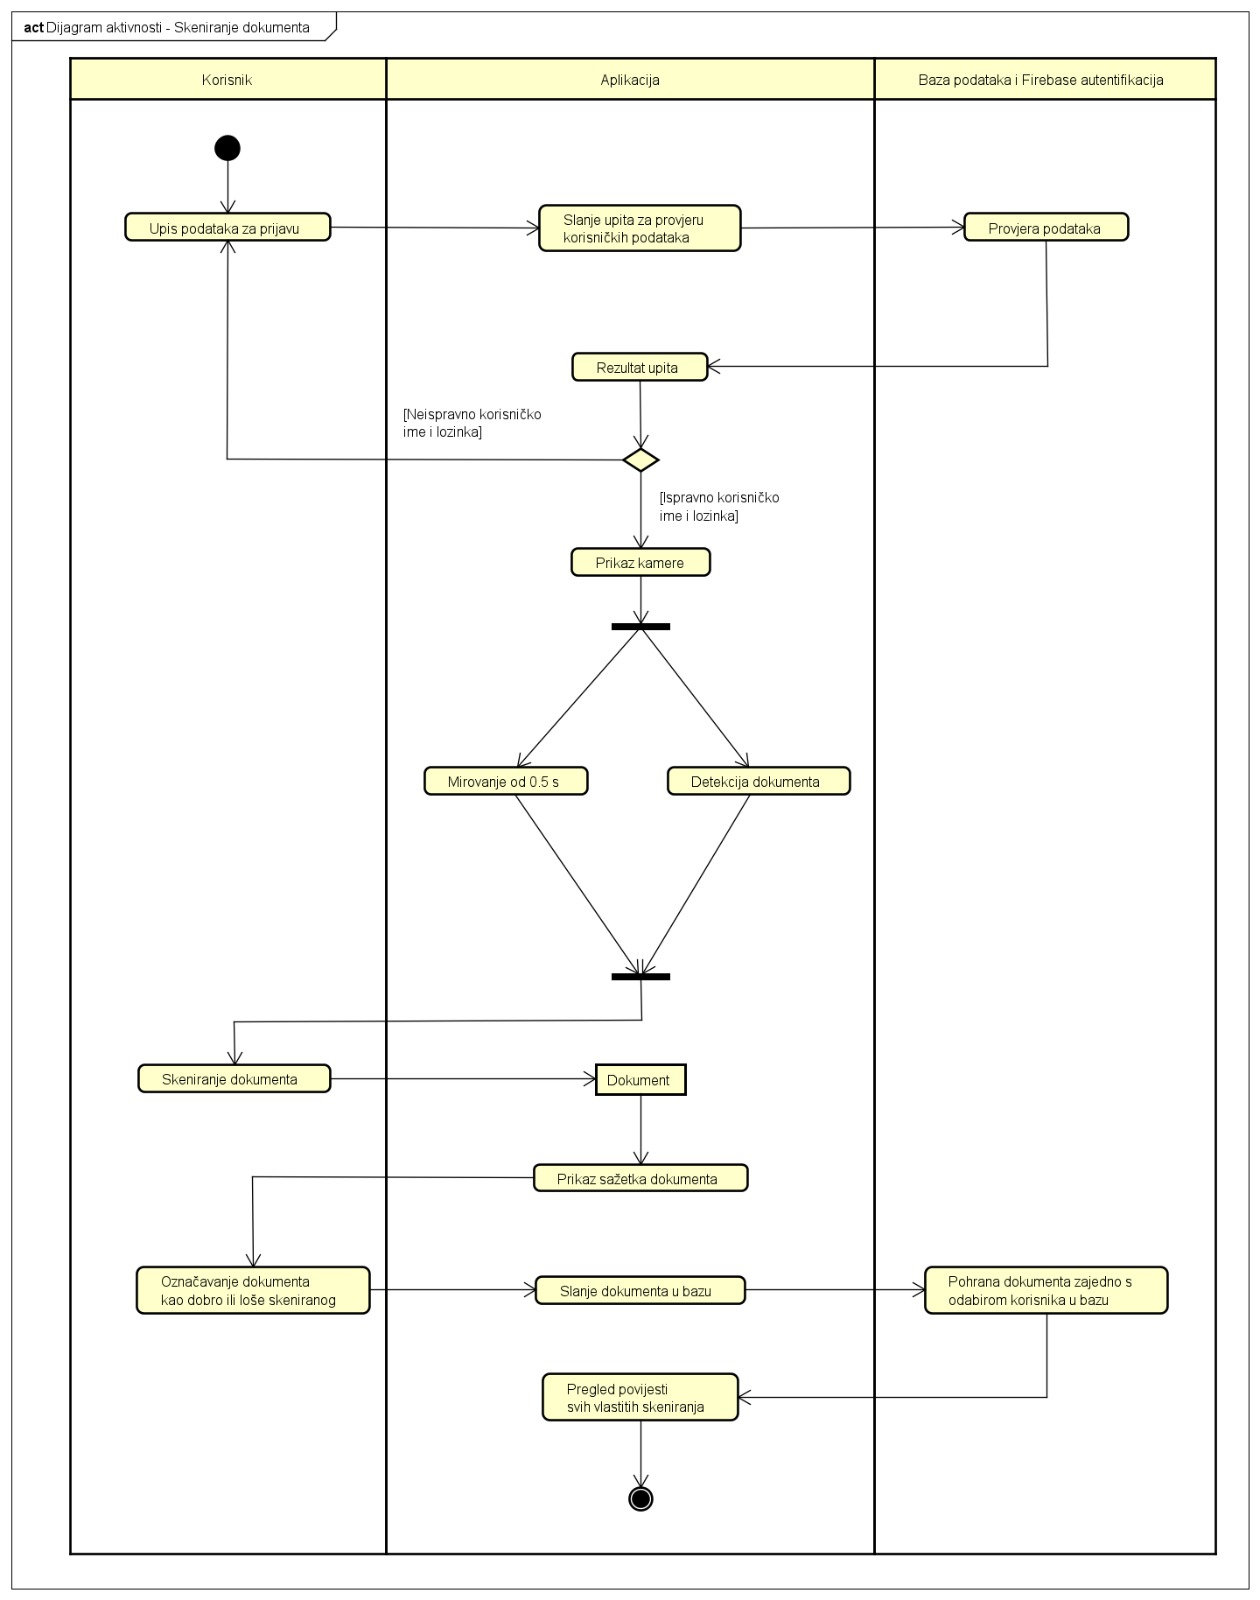
\includegraphics[width=\textwidth]{slike/Dijagram aktivnosti.jpeg}
				\caption{Dijagram aktivnosti - skeniranje dokumenta}
			\end{figure}
			
			\eject
		\section{Dijagram komponenti}
		
			\justify{Dijagram komponenti na slici 4.9. prikazuje unutarnju strukturu aplikacije i komunikaciju s Firebase uslugom koja aplikaciji pruža sve potrebne usluge kao što su NoSQL baza podataka, push obavijesti i autentifikacija korisnika. Aplikacija je modelirana po uzoru na MVVM arhitekturu stoga svako korisničko sučelje ima pripadni model koji njime upravlja. Češće korištene funkcije enkapsulirane su u helper komponente.\par
Prijava i registracija korisnika ostvarena je preko sučelja Auth pomoću Firebase biblioteke za autentifikaciju.\par
Model korisničkog sučelja koristi repozitorij kako bi aplikacija dohvatila ili spremila određene podatke koji se modeliraju pomoću skupa modela za dokumente i korisnike preko sučelja za NoSQL operacije.\par
Skeniranje dokumenata ostvareno je bibliotekom CameraX, a procesiranje skeniranih dokumenata izvodi se interno preko pripadnog sučelja pomoću Google ML Text Recognition biblioteke.\par
Komponenta zadužena za push obavijesti konstantno sluša Firebase dolazne poruke preko sučelja za poruke te ih šalje drugim komponentama aplikacije na prikaz.}
		
			 \begin{figure}[H]
				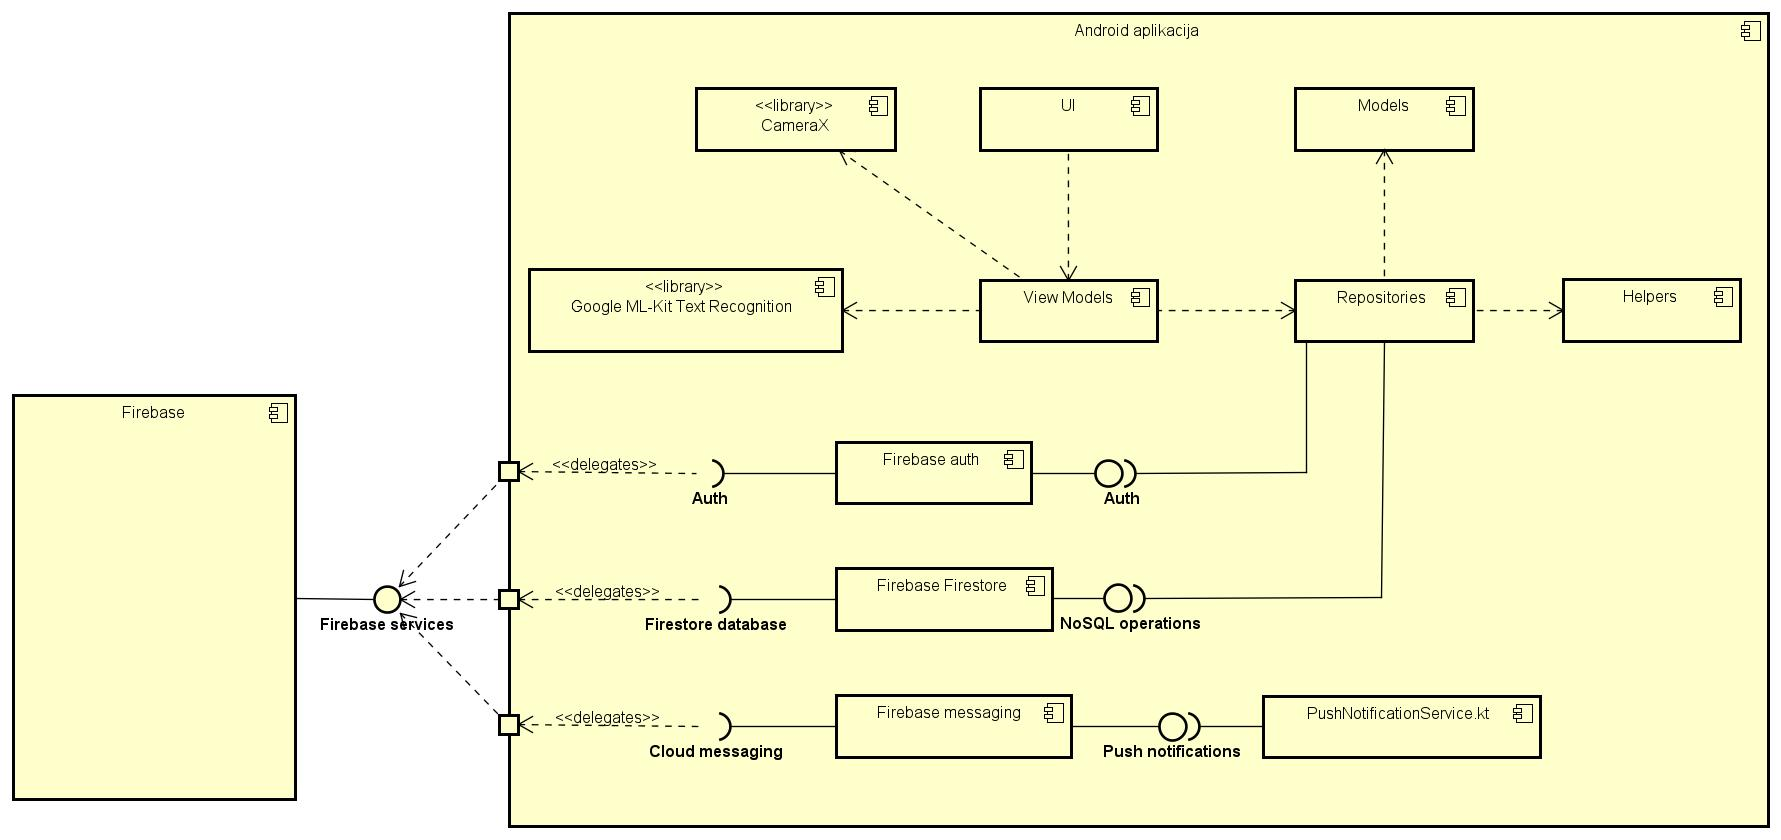
\includegraphics[width=\textwidth]{slike/Dijagram_komponenti.jpg}
				\caption{Dijagram komponenti}
			\end{figure}
	\chapter{Implementacija i korisničko sučelje}
		
		
		\section{Korištene tehnologije i alati}
		
		Komunikacija u timu ostvarena je korištenjem aplikacija \underline{Whatsapp}\footnote{\url{https://www.whatsapp.com}} i \underline{Discord}\footnote{\url{https://discord.com}}. 
		Za upravljanje izvornim kodom korišten je sustav \underline{Git}\footnote{\url{https://git-scm.com}}, a udaljeni repozitorij dostupan je na web platformi \underline{GitLab}\footnote{\url{https://about.gitlab.com}}. 
		Za izradu UML dijagrama iskoristili smo alat \underline{Astah}\footnote{\url{https://astah.net}}.

		Razvojno okruženje korišteno u Android dijelu aplikacije je \underline{Android Studio}\footnote{\url{https://developer.android.com/studio}} - integrirano 
		razvojno okruženje (IDE) kreirano na temeljima drugog JetBrainsovog IDE-a, IntelliJa. Također službeni je Googleov IDE za razvoj Android aplikacija, a rad u njemu je moguć
		u sva tri glavna operacijska sustava (Windows, Linux, MacOS).
		
		Za backend dio programskog koda korišten je Microsoftov uređivač teksta \underline{Visual} \underline{Studio} \underline{Code}\footnote{\url{https://code.visualstudio.com}}. 
		Iako je samo uređivač teksta,
		VSC, zahvaljujući mnoštvu plugina razvijenih od programerske zajednice, podsjeća na razvojno okruženje. U njemu je integriran i sustav Git što nam je olakšalo rad.

		Aplikacija je napisana za Android operacijski sustav s podrškom za verzije 10, 11, 12 koristeći programski jezik \underline{Kotlin}\footnote{\url{https://kotlinlang.org}}, 
		a cloud funkcije za bazu podataka Firebase pisane su u \underline{Node.js}\footnote{\url{https://nodejs.org}}, \underline{Javascript}\footnote{\url{https://www.javascript.com}}
		frameworku za izradu backenda. Node.js vrti se na V8 engineu te izvršava JavaScript kod izvan preglednika. Primarno služi za razvoj serverske strane web stranica
		za prikazivanje dinamičkog sadržaja, ali može poslužiti u bilo kojem dijelu serverskog programiranja. 

		Baza podataka se nalazi na Googleovom poslužitelju i razvijana je pomoću \underline{Firebase}\footnote{\url{https://firebase.google.com}} Google platforme.
		Firebase se koristi za praćenje analitike, prijavljivanje i popravljanje rušenja aplikacija, a ima ugrađene baze podataka (Realtime i Firestore).

		Unit testiranje smo vršili pomoću \underline{Mockito}\footnote{\url{https://site.mockito.org}} \textit{frameworka} koji je razvijan pod MIT licencom. Programski jezik korišten
		za testiranje je Kotlin.
		
			
			\eject 
		
	
		\section{Ispitivanje programskog rješenja}
			
			\subsection{Ispitivanje komponenti}
			\justify{Napravljena su 4 testa za AuthenticationViewModel:\newline
			\textbf{loginFakeUser()} provjerava error handling za pokušaj prijave nepostojećeg korisnika\newline
			\textbf{loginEmptyEmail()} provjerava error handling za pokušaj prijave s praznim email-om\newline
			\textbf{registerEmptyEmail()} provjerava error handling za pokušaj registracije s praznim email-om\newline
			\textbf{logout()} provjerava error handling za pokušaj odjave bez prijavljenog korisnika}
			
			\begin{figure}[H]
				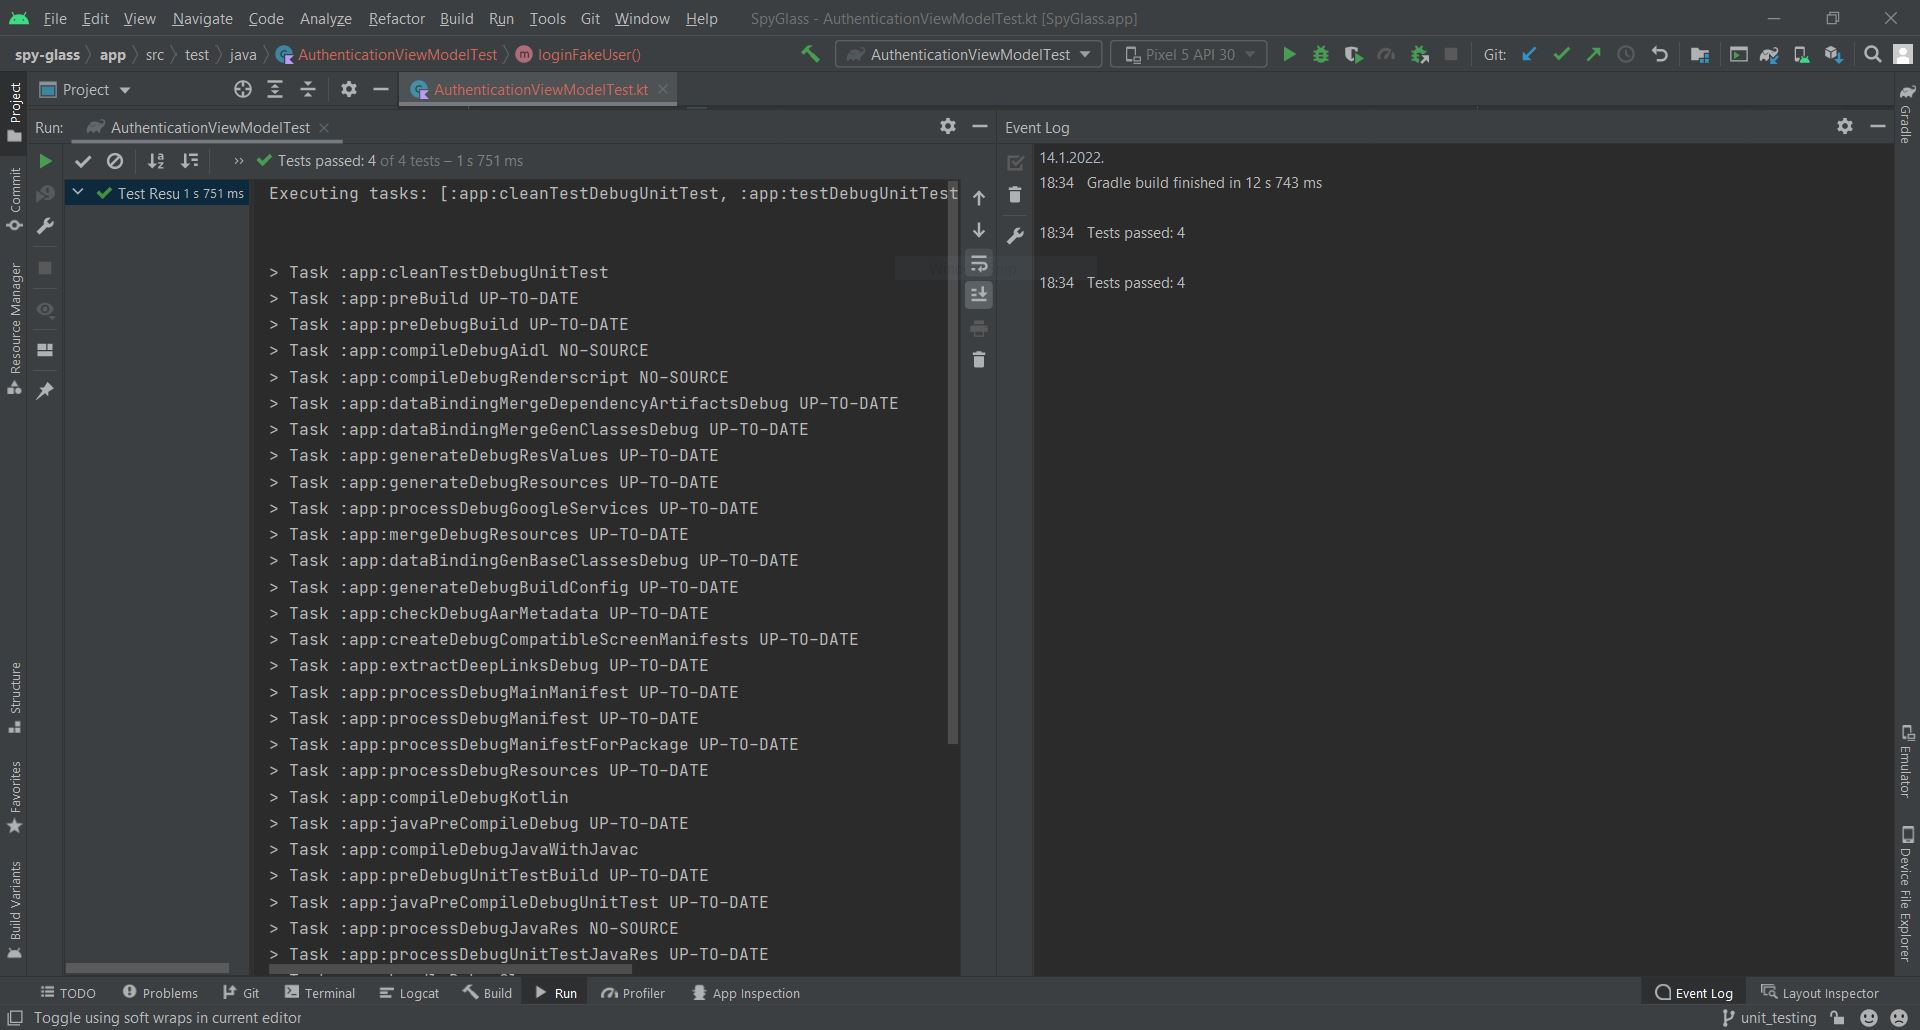
\includegraphics[width=\textwidth]{slike/testResultsAuth.jpg}
				\caption{Rezultati testova - AuthenticationViewModelTests}
			\end{figure}
			
			\begin{figure}[H]
				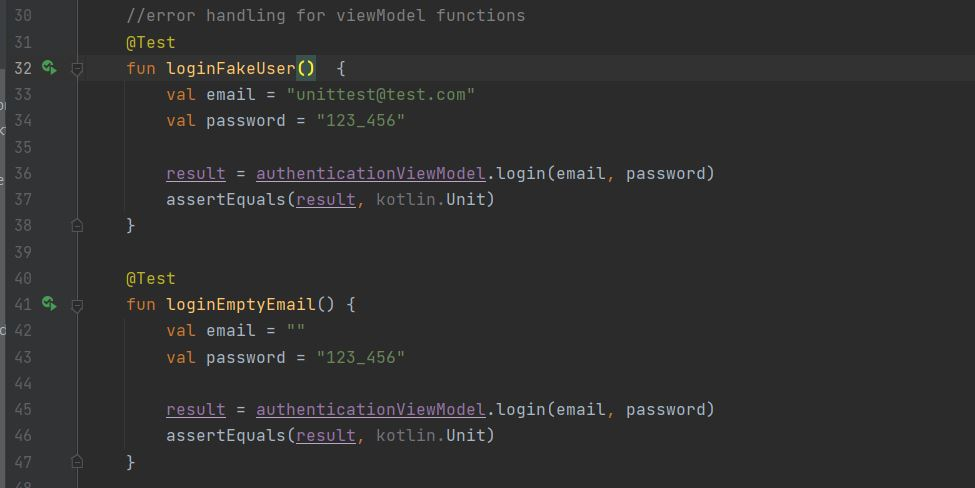
\includegraphics[width=\textwidth]{slike/authTests1.jpg}
				\caption{Isječak koda - AuthenticationViewModelTests}
			\end{figure}
			
			\begin{figure}[H]
				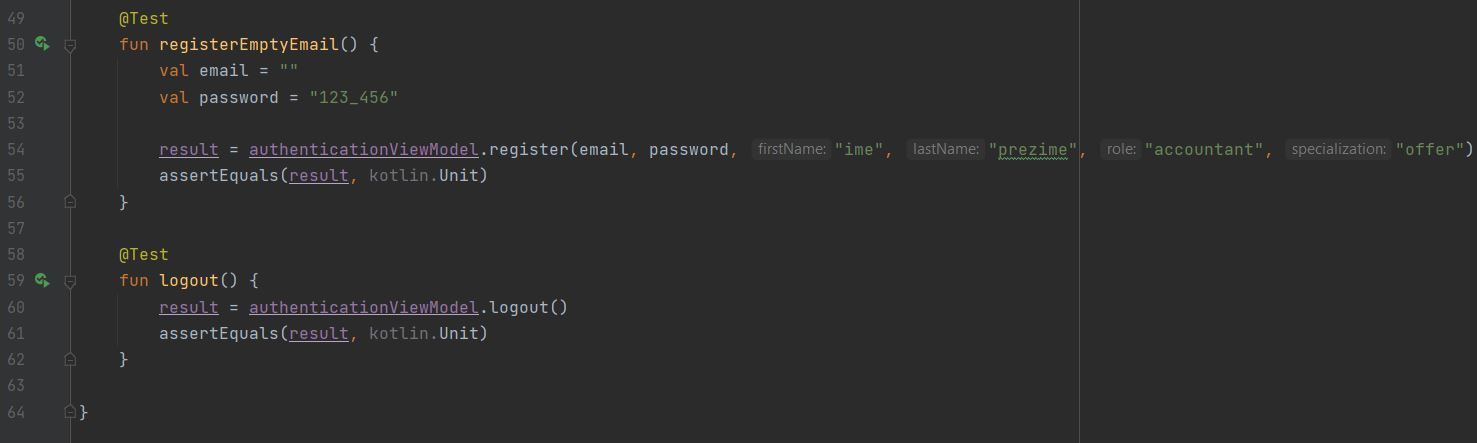
\includegraphics[width=\textwidth]{slike/authTests2.jpg}
				\caption{Isječak koda - AuthenticationViewModelTests}
			\end{figure}
			
			\justify{Napravljena su 2 testa za DocumentsViewModel:\newline
			\textbf{getDocumentsByFakeUser()} provjerava error handling za pokušaj dohvata dokumenata nepostojećeg korisnika\newline
			\textbf{getDocumentsLiveDataTest()} provjerava inicijalizaciju varijable documentsLiveData: MutableLiveData\textless List\textless Document\textgreater \textgreater}\\
			
			\begin{figure}[H]
				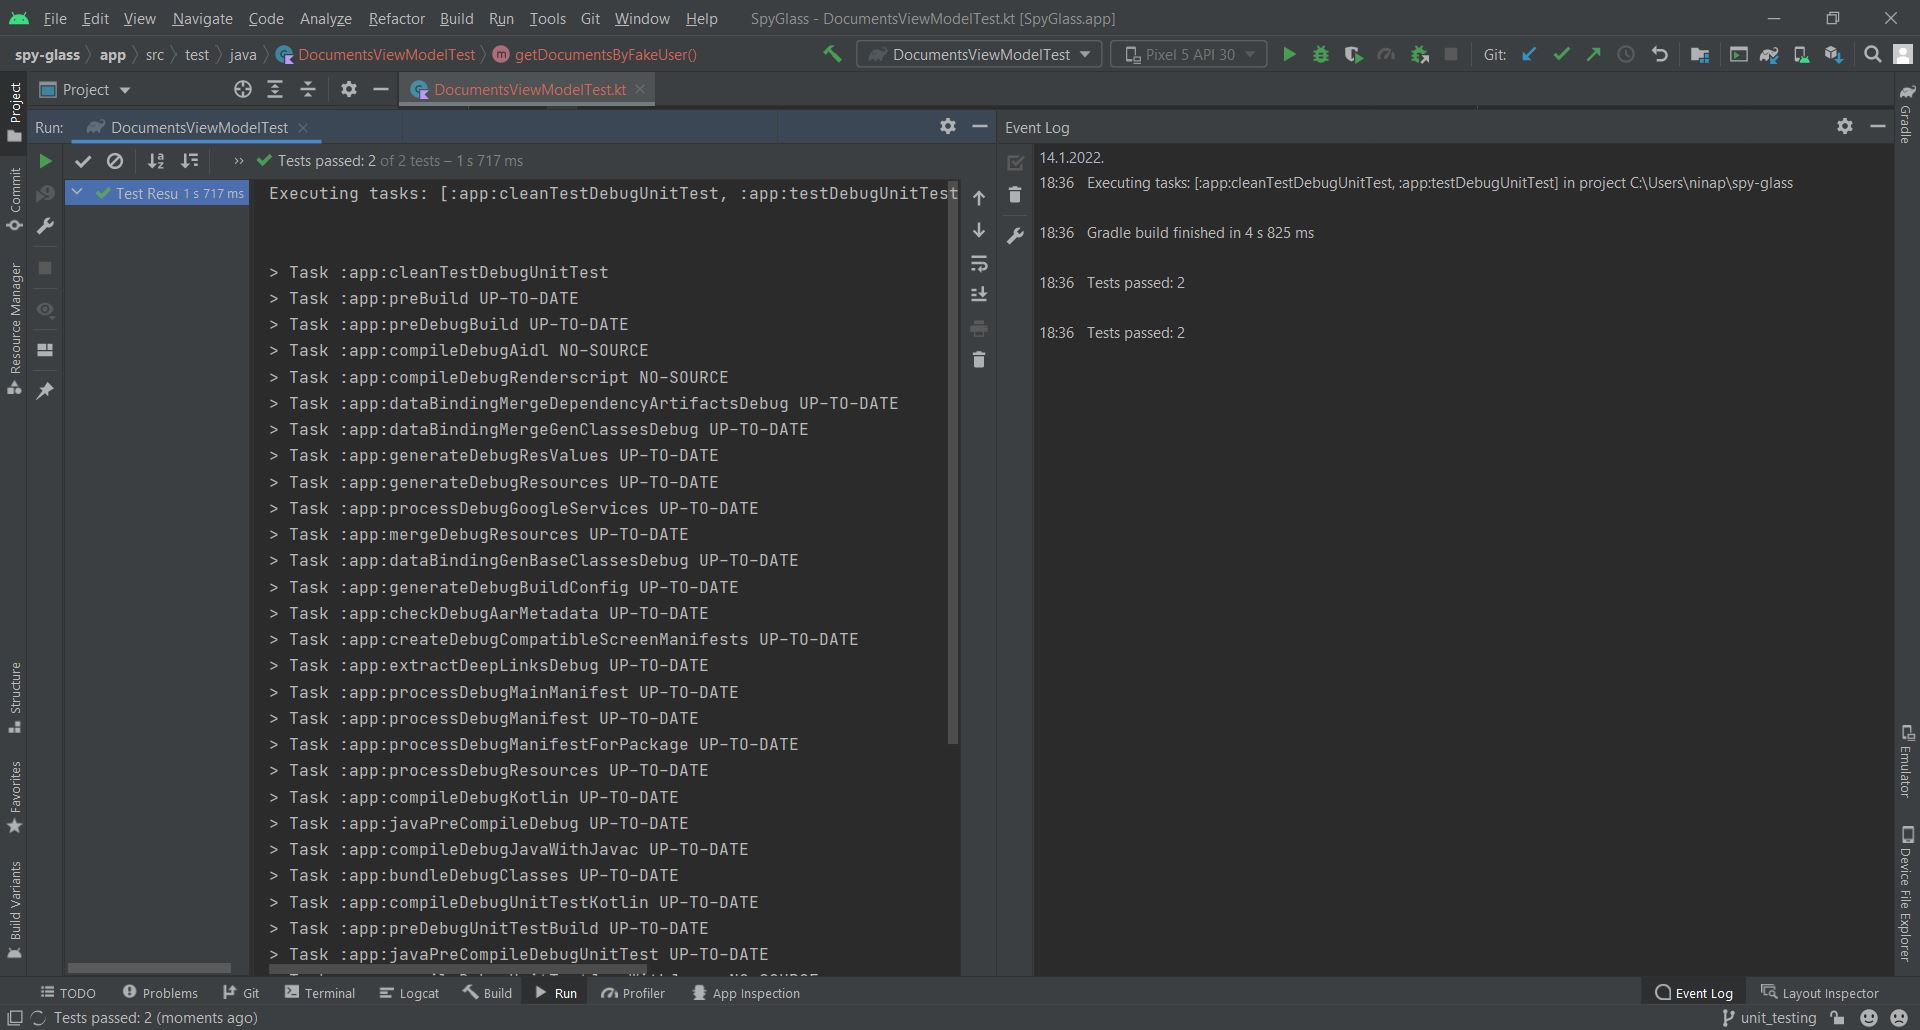
\includegraphics[width=\textwidth]{slike/testResultsDocs.jpg}
				\caption{Rezultati testova - DocumentsViewModelTests}
			\end{figure}
			
			\begin{figure}[H]
				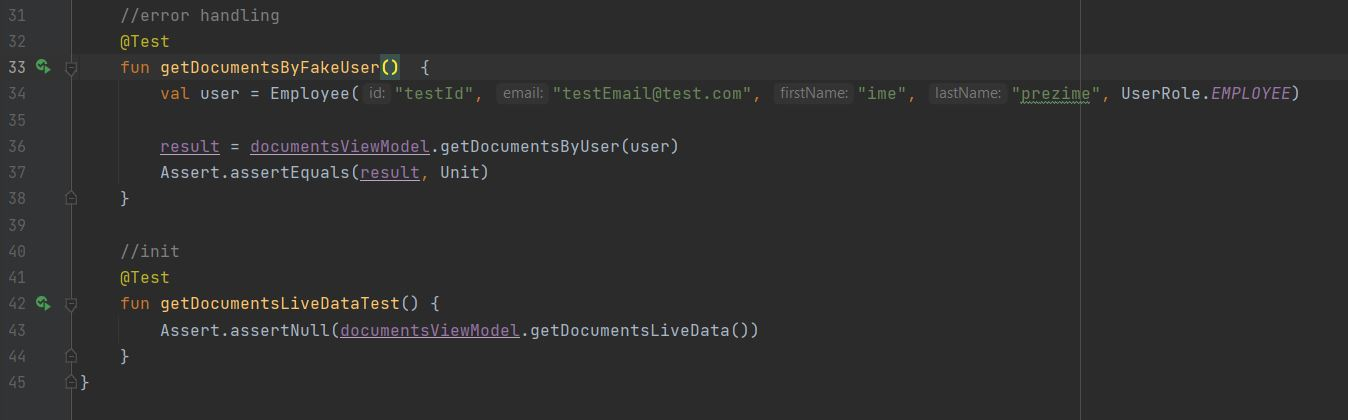
\includegraphics[width=\textwidth]{slike/documentsTests.jpg}
				\caption{Isječak koda - DocumentsViewModelTests}
			\end{figure}
			
			\subsection{Ispitivanje sustava}
			\justify{Svaki dio sustava ispitan je ručno po obrascima uporabe kako bi se pronašla neočekivana ponašanja aplikacije. Prikazan je dio ispitivanja sustava zbog jednostavnosti (UC1 - Registracija).
			\newline
			\newline
			\newline
			\textbf{Ispitni slučaj 1: Ispitivanje registracije direktora\newline
			Ulaz:\newline}
			1. Otvaranje aplikacije\newline
			2. Upisivanje identifikacijskih podataka\newline
			3. Pritiskanje gumba za registraciju 
			\newline
			\textbf{Očekivani rezultat:}
			\newline
			1. Prikazuje se zaslon za registraciju\newline
			2. Provjera formata unosa\newline
			3. Pošalji podatke i prihvati registraciju
			\newline
			\textbf{Rezultat: } Očekivanja su zadovoljena. Aplikacija je prošla test.
			}
			\begin{figure}[H]
				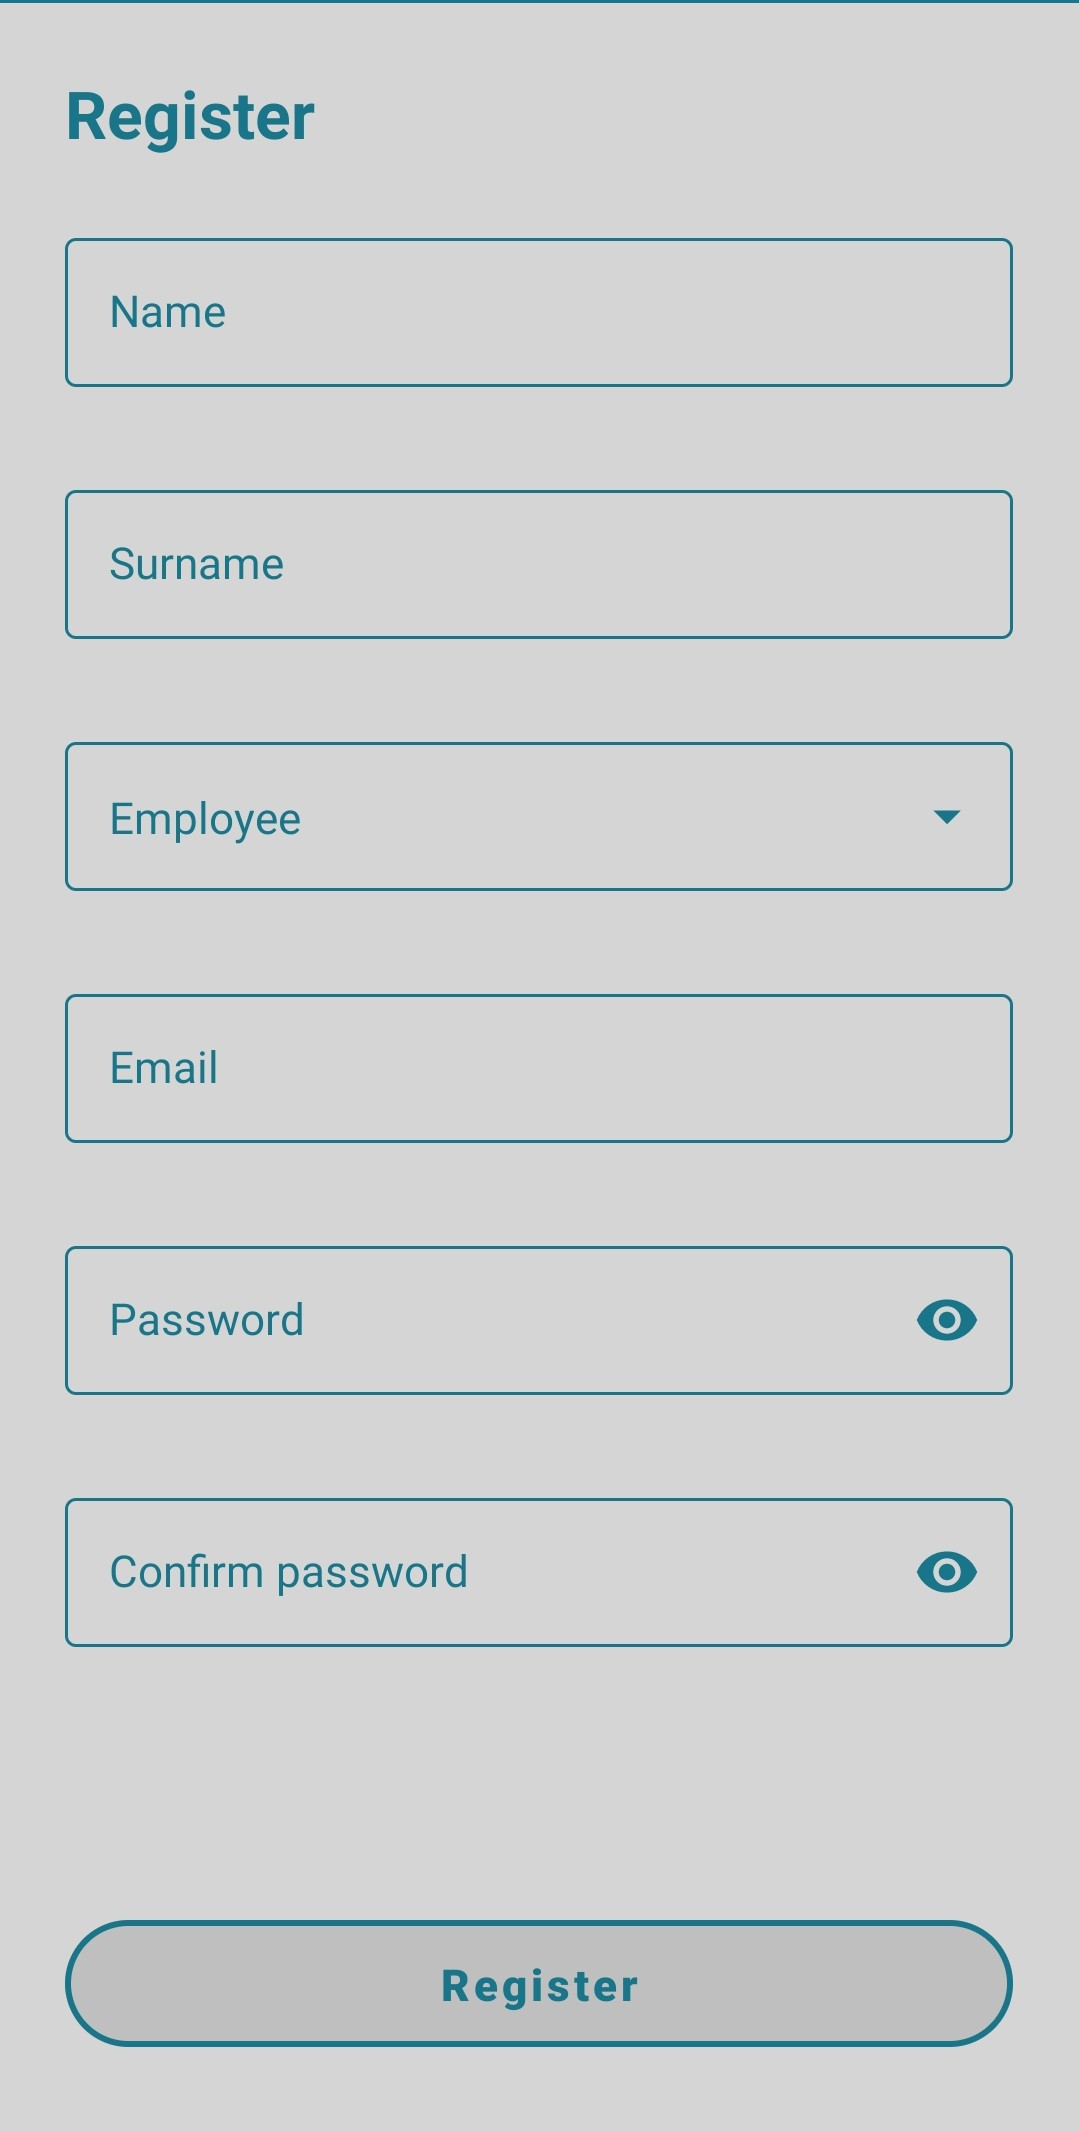
\includegraphics[scale=0.25]{slike/register.jpg}
				\caption{Zaslon za registraciju}
			\end{figure}
			
			\eject 
		
		
		\section{Dijagram razmještaja}
			
			 	\justify{Dijagram razmještaja je strukturni statički UML dijagram koji opisuje topologiju sustava i usredotočen je na odnos sklopovskih i programskih dijelova. Na slici 5.7 prikazan je specifikacijski dijagram razmještaja. Specifikacijski dijagram prikazuje pregled implementacije artefakata bez upućivanja na specifične slučajeve artefakata ili čvorova. Na poslužiteljskom računalu se nalazi poslužitelj baze podataka. Klijent koristi mobilnu aplikaciju namijenjenu za operacijski sustav Android. Komunikacija između klijenta i baze podataka odvija se preko protokola HTTP.}\\
			 
			 \begin{figure}[H]
			 	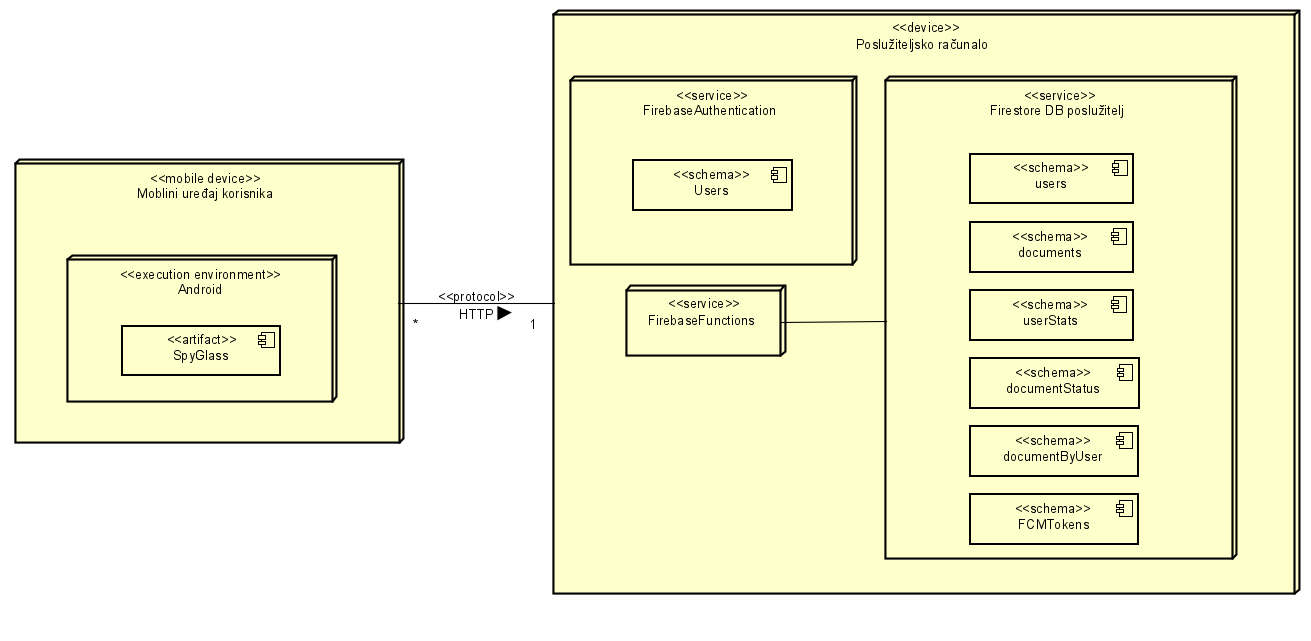
\includegraphics[width=\textwidth]{slike/Dijagram_razmjestaja.png}
			 	\caption{Dijagram razmještaja}
			 \end{figure}
			
			\eject 
		
		\section{Upute za puštanje u pogon}

		\subsection{Kreiranje projekta i integracija SDK-a u Android}
		\begin{packed_enum}
			\item Kreirati Firebase projekt
				\begin{packed_enum}
					\item Imenovati projekt
					\item Omogućiti \textbf{Google Analytics}
					\item Kliknuti \textbf{Create project}
				\end{packed_enum}
	
			\item Registrirati aplikaciju
				\begin{packed_enum}
					\item Kliknuti opciju \textbf{Add app}
					\item Unijeti Android package name koji odgovara imenu od aplikacije
					\item Kliknuti \textbf{Register app}
				\end{packed_enum}
	
			\item Dodati Firebase configuration datoteku u aplikaciju
				 \begin{packed_enum}
					\item Preuzeti \textbf{google-services.json} iz Firebase konzole
					\item Staviti datoteku u ispravni direktorij (module ili app-level direktorij)
					\item Dodati u \textbf{build.gradle} datoteku koja se nalazi u root-level ili project-level direktoriju navedeni tekst:
						\begin{lstlisting}[mathescape=true,breaklines=true,autogobble=true]
							buildscript {
	
								repositories {
									// Check that you have the following line (if not, add it):
									google()  // Google's Maven repository
								}
	
								dependencies {
									// ...
	
									// Add the following line:
									classpath 'com.google.gms:google-services:4.3.10'  // Google Services plugin
								}
							}
	
								allprojects {
								// ...
	
									repositories {
										// Check that you have the following line (if not, add it):
										google()  // Google's Maven repository
										// ...
									}
								}
						\end{lstlisting}
					\item Dodati u \textbf{build.gradle} datoteku koja se nalazi u module ili app-level direktoriju navedeni tekst:
						\begin{lstlisting}[mathescape=true,breaklines=true,autogobble=true]
							apply plugin: 
							'com.android.application'
							// Add the following line:
							apply plugin: 'com.google.gms.google-services'  // Google Services plugin
	
							android {
							// ...
						}
						\end{lstlisting}
				\end{packed_enum}
	
			\item Dodati Firebase SDK u aplikaciju
				\begin{packed_enum}   
					\item Dodati u \textbf{build.gradle} datoteku koja se nalazi u module ili app-level direktoriju navedeni tekst:      
						\begin{lstlisting}[mathescape=true,breaklines=true,autogobble=true]
							dependencies {
							// ...
				  
							// Import the Firebase BoM
							implementation platform('com.google.firebase:firebase-bom:29.0.3')
				  
							// When using the BoM, you don't specify versions in Firebase library dependencies
				  
							// Declare the dependency for the Firebase SDK for Google Analytics
							implementation 'com.google.firebase:firebase-analytics-ktx'
				  
							// Declare the dependencies for any other desired Firebase products
							// For example, declare the dependencies for Firebase Authentication and Cloud Firestore
							implementation 'com.google.firebase:firebase-auth-ktx'
							implementation 'com.google.firebase:firebase-firestore-ktx'
						  }
						\end{lstlisting} 
					\item Kliknuti gumb \textbf{Sync} u programu Android Studio kako bi svi \textbf{dependencies} bili na najnovijoj verziji
				\end{packed_enum} 
	
			\item U Firebase konzoli omogućiti authentifikaciju preko email adrese i lozinke
				\begin{packed_enum}
					\item Otvoriti \textbf{Auth} sekciju unutar konzole
					\item Pod \textbf{Sign in method} odabrati opciju \textbf{Email/password} i kliknuti gumb \textbf{Save}
				\end{packed_enum}
	
			\item Dodati \textbf{dependencies} za Firebase authentifikaciju
				\begin{packed_enum}
					\item Dodati u \textbf{build.gradle} datoteku koja se nalazi u module ili app-level direktoriju navedeni tekst:
					\begin{lstlisting}[mathescape=true,breaklines=true,autogobble=true]
						dependencies {
							// Import the BoM for the Firebase platform
							implementation platform('com.google.firebase:firebase-bom:29.0.3')
				
							// Declare the dependency for the Firebase Authentication library
							// When using the BoM, you don't specify versions in Firebase library dependencies
							implementation 'com.google.firebase:firebase-auth-ktx'
						}
					\end{lstlisting}
				\end{packed_enum}
		\end{packed_enum}	 
		
		\subsection{Puštanje u pogon Cloud Funkcija}
		\justify{
			\textbf{Cloud Functions} služe za automatsko pokretanje pozadinskog koda kao odgovor na događaje koje pokreću značajke Firebasea, primjerice triggeri kolekcija u bazi podataka. 
		Nakon kreiranja Firebase projekta, opisanog u prethodnom dijelu teksta potrebni su sljedeći koraci:}
		\begin{packed_enum}
			\item Instalacija node.js i Firebase CLI-a. Potrebno je instalirati i npm, te pokrenuti sljedeću naredbu:
				\begin{lstlisting}[mathescape=true,breaklines=true,autogobble=true]
					npm install -g firebase-tools
				\end{lstlisting}
			\item Povezati projekt lokalno s cloudom:
				\begin{lstlisting}[mathescape=true,breaklines=true,autogobble=true]
					firebase login
					firebase init firestore
					firebase init functions
				\end{lstlisting}
			\item Napisati Cloud funkciju te pokrenuti
				\begin{lstlisting}[mathescape=true,breaklines=true,autogobble=true]
					firebase deploy --only functions
				\end{lstlisting}
		\end{packed_enum}

		\subsection{Pokretanje Android aplikacije}
		\justify{Potrebno je preuzeti spyglass.apk datoteku s Gitlab repozitorija projekta pod direktorijem \textit{apk} na mobilni uređaj. 
		Zatim ju je potrebno pokrenuti čime će se pokrenuti i instalacija Android aplikacije nakon čega klikom na ikonu aplikacije
		pokrećemo aplikaciju.}
			
			\eject 
	\chapter{Zaključak i budući rad}
		
\justify{Zadatak zadan ovim projektom dovoljno je složen kako bi se članovi tima s nikakvim do malim iskustvom upoznali s mnogim problemima organizacije 
posla i vremena, programiranja, dizajna sustava i komunikacije unutar tima te tako dobili dojam o pravim problemima koje je potrebno rješiti kod
 razvoja programske podrške za stvarne klijente. Unatoč ambicioznom početku, većina članova tima su inicijalno slabo bili upoznati s razvojem
  programske podrške za sustav Android što je dodalo dodatnu razinu kompleksnosti na zadatak. Zajedničkim radom i suradnjom, projekt je u
   predefiniranom roku uspješno završen i tim je zadovoljan rezultatom.\par

Nakon sastavljanja tima, članovi tima krenuli su se upoznavati sa Android sustavom
 i alatima za razvoj programske podrške kao što je Git, Android studio i programski
  jezik Kotlin i sl. Nakon shvaćenog opsega projekta, članovi tima podijelili su se
   na zadatke koji najbolje odgovaraju sposobnostima pojedinog člana. Voditelj tima pratio je napredak svakog člana te 
   uskakao u pomoć ukoliko je to bilo potrebno. Iskusniji članovi tima izradili su kostur aplikacije dok su se ostali članovi posvetili 
   proučavanju zadatka u detalje i izradi tehničke dokumentacije kako bi za početak implementacije funkcionalnosti tim imao dobru podlogu.\par

Prva funkcionalnost koja je razvijena je sustav za registraciju i prijavu korisnika. Budući da je korištena dobro poznata i dokumentirana usluga 
Firebase, ova faza implementacije prošla je bez većih poteškoća.\par

Sljedeća funkcionalnost koja je implementirana je pospremanje tokena za push obavijesti u bazu podataka koja nije u cijelosti dokumentirana od 
strane Firebase usluge. Posljedica je funkcionalni sustav koji nije ostvaren najefikasnije moguće i podložan problemima kod proširenja aplikacije.\par

Naš najveći izazov bio je implementirati dinamičku detekciju dokumenta. Uspjeli smo to izvesti korištenjem Google-ovog ML Kita s kojim unutar 
implementacije CameraX API-ja provjeravamo je li na ekranu zapravo dokument. Osim toga nismo imali značajnijih izazova te su sve tražene funkcionalnosti
implementirane.

Projekt bi bio završen ranije da smo imali više iskustva s radom u timu te iskustva s radom u Androidu. No s vremenom je tim postao sve bolji te
smo brže i kvalitetnije implementirali tražene značajke.

Rad na projektu pokazao se dovoljno izazovnim da svaki od članova tima steče nova znanja o tehnologijama, timskom radu i svojim sposobnostima, a
u isto vrijeme dovoljno jednostavan da se tim rastane sa zadovoljstvom i iskustvom koje će im u budućoj karijeri olakšati prilagodbu ozbiljnom zadatku.

}
		
		\eject 
	\chapter*{Popis literature}
		\addcontentsline{toc}{chapter}{Popis literature}		
		
		\begin{enumerate}
			
			\item  M. Moskala, I. Wojda, "Android Development with Kotlin", Packt Publishing Ltd., 2017

			\item  UML Use Case Diagram Tutorial, \url{https://www.lucidchart.com/pages/uml-use-case-diagram}
			
			\item  Learn Git Branching, \url{https://learngitbranching.js.org/}
	
			\item  Guide to app architecture, \url{https://developer.android.com/jetpack/guide}

			\item  Model-View-ViewModel (MVVM) Explained, \url{https://www.wintellect.com/model-view-viewmodel-mvvm-explained/}

			\item  Handling Lifecycles with Lifecycle-Aware Components, \url{https://developer.android.com/topic/libraries/architecture/lifecycle}

			\item  Saving UI States, \url{https://developer.android.com/topic/libraries/architecture/saving-states}

			\item  Handle configuration changes, \url{https://developer.android.com/guide/topics/resources/runtime-changes}

			\item  Firebase Documentation, \url{https://firebase.google.com/docs}

			\item  CameraX overview, \url{https://developer.android.com/training/camerax}

			\item  Recognize text in images with ML Kit on Android, \url{https://developers.google.com/ml-kit/vision/text-recognition/android}

			\item  Kotlin coroutines on Android, \url{https://developer.android.com/kotlin/coroutines}

		\end{enumerate}
		
		 
	
	\begingroup
	\renewcommand*\listfigurename{Indeks slika i dijagrama}
	%\renewcommand*\listtablename{Indeks tablica}
	%\let\clearpage\relax
	\listoffigures
	%\vspace{10mm}
	%\listoftables
	\endgroup
	\addcontentsline{toc}{chapter}{Indeks slika i dijagrama}


	
	\eject 
		
	\chapter*{Dodatak: Prikaz aktivnosti grupe}
		\addcontentsline{toc}{chapter}{Dodatak: Prikaz aktivnosti grupe}
		
		\section*{Dnevnik sastajanja}
		
		\begin{packed_enum}
			\item  sastanak
			
			\item[] \begin{packed_item}
				\item Datum: 13. listopada 2021.
				\item Prisustvovali: Ivan Futivić, Karlo Marković, Rafael Boban, Blaž Solić, Nina Petrušić, Luka Hanžek
				\item Teme sastanka:
				\begin{packed_item}
					\item  prvi sastanak s asistentom i timom
					\item  diskusija o projektu i zadanom zadatku s visokog pogleda
					\item  diskusija o tehnologijama prikladnim za projektni zadatak
					\item  međusobno upoznavanje
				\end{packed_item}
			\end{packed_item}
			
			\item  sastanak
			\item[] \begin{packed_item}
				\item Datum: 19. listopada 2021.
				\item Prisustvovali:  Ivan Futivić, Karlo Marković, Rafael Boban, Karlo Kada, Nina Petrušić, Luka Hanžek
				\item Teme sastanka:
				\begin{packed_item}
					\item  specifikacija programske potpore
					\item  detaljna razrada zadatka
					\item  izgled baze podataka
					\item  diskutiranje o potencijalnim rješenjima
					\item  upoznavanje s NoSQL bazom podataka
					\item  diskutiranje o sustavu za slanje obavijesti
				\end{packed_item}
			\end{packed_item}
			
			\item  sastanak
			\item[] \begin{packed_item}
				\item Datum: 2. studenog 2021.
				\item Prisustvovali:  Ivan Futivić, Rafael Boban, Blaž Solić, Karlo Kada, Luka Hanžek
				\item Teme sastanka:
				\begin{packed_item}
					\item  specifikacija programske potpore
					\item  struktura baze podataka
					\item  rješavanje nedoumica u dizajnu i zahtjevima
					\item  podjela poslova
					\item  arhitektura sustava
				\end{packed_item}
			\end{packed_item}
			
			\item  sastanak
			\item[] \begin{packed_item}
				\item Datum: 9. studenog 2021.
				\item Prisustvovali:  Ivan Futivić, Karlo Marković, Blaž Solić, Karlo Kada, Nina Petrušić, Luka Hanžek
				\item Teme sastanka:
				\begin{packed_item}
					\item  diskutiranje o dovršavanju dokumentiranja prve revizije projekta
					\item  rješavanje nedoumica u dizajnu i zahtjevima
					\item  prilagođavanje prvobitnog plana podjele posla
				\end{packed_item}
			\end{packed_item}
			
			\item  sastanak
			\item[] \begin{packed_item}
				\item Datum: 6. prosinca 2021.
				\item Prisustvovali:  Ivan Futivić, Karlo Marković, Blaž Solić, Karlo Kada, Nina Petrušić, Luka Hanžek
				\item Teme sastanka:
				\begin{packed_item}
					\item  rasprava o načinu ponašanja obavijesti
					\item  priprema za prvo kolokviranje
					\item  podjela ostatka posla vezano za aplikaciju
				\end{packed_item}
			\end{packed_item}

			\item  sastanak
			\item[] \begin{packed_item}
				\item Datum: 20. prosinca 2021.
				\item Prisustvovali:  Ivan Futivić, Karlo Marković, Blaž Solić, Karlo Kada, Rafael Boban
				\item Teme sastanka:
				\begin{packed_item}
					\item  podjela posla za završne dijelove dokumentacije
					\item  priprema za odmor tijekom blagdana
				\end{packed_item}
			\end{packed_item}

			\item  sastanak
			\item[] \begin{packed_item}
				\item Datum: 10. siječnja 2022.
				\item Prisustvovali:  Ivan Futivić, Karlo Marković, Blaž Solić, Karlo Kada, Rafael Boban, Nina Petrušić, Luka Hanžek
				\item Teme sastanka:
				\begin{packed_item}
					\item  dovršavanje dokumentacije
					\item  popravljanje bugova u dokumentaciji
					\item  finaliziranje koda 
					\item  razgovor o izradi prezentacije
					\item  testiranje koda
				\end{packed_item}
			\end{packed_item}
			
		\end{packed_enum}
		
		\eject
		\section*{Tablica aktivnosti}

			\begin{longtblr}[
					label=none,
				]{
					vlines,hlines,
					width = \textwidth,
					colspec={X[7, l]X[1, c]X[1, c]X[1, c]X[1, c]X[1, c]X[1, c]X[1, c]}, 
					vline{1} = {1}{text=\clap{}},
					hline{1} = {1}{text=\clap{}},
					rowhead = 1,
				} 
				\multicolumn{1}{c|}{} & \multicolumn{1}{c|}{\rotatebox{90}{\textbf{Ivan Futivić}}} & \multicolumn{1}{c|}{\rotatebox{90}{\textbf{Rafael Boban }}} &	\multicolumn{1}{c|}{\rotatebox{90}{\textbf{Karlo Marković }}} & \multicolumn{1}{c|}{\rotatebox{90}{\textbf{Blaž Solić }}} &	\multicolumn{1}{c|}{\rotatebox{90}{\textbf{Karlo Kada }}} & \multicolumn{1}{c|}{\rotatebox{90}{\textbf{Nina Petrušić }}} &	\multicolumn{1}{c|}{\rotatebox{90}{\textbf{Luka Hanžek }}} \\  
				Upravljanje projektom 			&4  &0  &0  &0  &0  &0  &0 \\ 
				Opis projektnog zadatka 		& 0 &0  &0  &0  &0  &0  &3 \\ 
				
				Funkcionalni zahtjevi       	&0  &0  &0  &1  &0  &0  &0,2  \\ 
				Opis pojedinih obrazaca 		&0  &0  &0  &1  &0  &0  &4  \\ 
				Dijagram obrazaca 				&0  &0  &0  &1  &0  &0  &3  \\ 
				Sekvencijski dijagrami 			&0  &0  &0  &0  &0  &0  &3  \\ 
				Opis ostalih zahtjeva 			&0,25  &0  &0  &0  &0  &0  &0,5  \\ 

				Arhitektura i dizajn sustava	 	&5  &5  &0  &1  &0  &0  &0  \\ 
				Baza podataka				        &6  &0  &0  &4  &0  &0  &0   \\ 
				Dijagram razreda 				    &0,2  &0  &8  &0  &0  &0  &0  \\ 
				Dijagram stanja				        &0  &0  &0  &1  &0  &0  &0  \\ 
				Dijagram aktivnosti 				&0  &0  &0  &0  &2  &0  &0  \\ 
				Dijagram komponenti			        &0  &0  &0  &0  &0  &0  &3  \\ 
				Korištene tehnologije i alati 		&0,5  &0  &0  &0,5  &0  &0  &0  \\ 
				Ispitivanje programskog rješenja 	&0  &0  &0  &0  &0  &10  &0  \\ 
				Dijagram razmještaja			    &0  &0  &2  &0  &0  &0  &0  \\ 
				Upute za puštanje u pogon 		    &1  &0  &0  &1  &0  &0  &0  \\ 
				Dnevnik sastajanja 				    &2  &0  &0  &0  &0  &0  &0,5  \\ 
				Zaključak i budući rad 			    &0  &1  &0  &0  &0  &0  &0  \\  
				Popis literature 				    &0  &0 &0  &0  &0  &0  &1  \\ 
				&  &  &  &  &  &  &  \\ \hline 
				\textit{izrada predloška koda}					&0  &2  &0  &0  &0  &0  &0 \\  
				\textit{izrada login/register sustava} 			&10  &0  &0  &0  &0  &0  &0 \\  
				\textit{spajanje s bazom podataka} 				&1  &0  &0  &5  &0  &0  &0  \\ 
				\textit{izrada sustava za obavijesti}			&0,2  &0  &0  &0  &0  &0  &6 \\
				\textit{backend}    							&2  &0  &0  &2  &0  &2  &0 \\ 
				\textit{izgled aplikacije}						&2  &8  &0  &0  &0  &0  &0 \\
				\textit{izrada pretrage povijesti dokumenata}	&5  &14  &0  &0  &5  &0  &0 \\
				\textit{izrada pregleda osobnih podataka}		&0  &0  &8  &0  &0  &0  &0 \\
				\textit{izrada OCR skenera}						&0  &15  &0  &0 &0  &0  &0 \\
				\textit{izrada prikaza statistike}				&1  &2  &4  &0 &0  &0  &0 \\
				\textit{izrada modela}							&1  &0  &0 &1  &0  &4  &0	\\
			\end{longtblr}
					
					
		\eject
	


\end{document} %naredbe i tekst nakon ove naredbe ne ulaze u izgrađen dokument 


